\documentclass[a4paper,twoside]{blocksbook}
\usepackage[cm-default]{fontspec}% provides font selecting commands
\usepackage{xunicode}% provides unicode character macros
\usepackage{xltxtra} % provides some fixes/extras
\usepackage[answerdelayed,lastexercise]{exercise}
\usepackage[labelsep=period,labelfont=it,textfont=it]{caption}
\usepackage{pifont}  % provides access to weird PS font chars
\usepackage{alltt}
\usepackage{url}
\usepackage{listings} 
\usepackage{color}
\usepackage{graphicx}
\usepackage{relsize}
\usepackage{xCJK}
\usepackage{scalefnt}
\usepackage{wrapfig}
\usepackage{everypage}
% Tables from Gnumeric
\usepackage{array} 
\usepackage{longtable}
\usepackage{calc}
\usepackage{multirow}
\usepackage{hhline} 
\usepackage{ifthen} 

\usepackage{tikz}
\usetikzlibrary{arrows,decorations.pathreplacing}
\usepackage{float}

\defaultfontfeatures{Scale=MatchLowercase,Mapping=tex-text}
\setmainfont{Droid Serif}
\setsansfont{Droid Sans}
\setmonofont[SmallCapsFont={DejaVu Sans Mono},Scale=0.70]{DejaVu Sans Mono}
\def\inputGnumericTable{}

%% list of answers
\newlistof{listofex}{ex}{List of Exercises}
\newlistentry{exercise}{ex}{0}

%% does not work?
%% or \renewcommand*{\bibmark}{\markboth{\bibname}{}}
\renewcommand*{\bibmark}{\markboth{\bibname}{\bibname}}
\nobibintoc
\renewcommand*{\indexmark}{\markboth{\indexname}{\indexname}}
\noindexintoc
\makeindex

%%\DeclareCaptionFont{white}{\color{white}}
%%\DeclareCaptionFormat{listing}{\colorbox[cmyk]{0.43, 0.35,
%%0.35,0.01}{\parbox{0.5\textwidth}{\hspace{0.5em}#1#2#3}}} % 0.98 same as listings
%%\captionsetup[lstlisting]{format=listing,labelfont=white,textfont=white,singlelinecheck=false,margin=0em,font={bf,footnotesize}}

%% Listings
\lstdefinelanguage{Go}
  {morekeywords={break,cap,case,chan,const,continue,copy,default,defer,else,fallthrough,%
  for,func,go,goto,if,import,interface,len,make,map,package,range,return,select,%
  struct,switch,type,var,%  % types
  uint8,uint16,uint32,uint64,int8,int16,int32,int64,float32,float64,byte,%
  complex,complex32,complex64,%
  int,uint,float,bool,uintptr,string,%
  iota,%
  },%
  otherkeywords={<-,!,;,\{,\}},%  %% nog beter maken
    sensitive=true,%
    morecomment=[l]{//},%
    morecomment=[s]{/*}{*/},%
    morecomment=[n]{(*}{*)},%
    morestring=[b]",%
    morestring=[b]',%
  }[]%
\lstset{language=Go,inputencoding=utf8,extendedchars=false,texcl,escapechar=\|,basicstyle=\ttfamily,keywordstyle=\bfseries,numbers=none,numberblanklines=false,showstringspaces=false,breaklines=true,numberstyle=\tiny\ttfamily,xleftmargin=\parindent,xrightmargin=1em,linewidth=0.98\linewidth}

\renewcommand{\lstlistlistingname}{List of Go Code}
\newcommand{\coderemark}[1]{\qquad$\leftarrow \textit{\small #1}$}

%% Exercises
\renewcommand{\ExerciseHeaderTitle}{\ExerciseTitle}
\renewcommand{\ExerciseHeaderLabel}{}
\renewcommand{\ExerciseName}{}	%% was 'Exercise'
\renewcommand{\ExerciseHeaderNB}{\theExercise}
%% This one is actually used
\renewcommand{\ExerciseHeader}{\vspace{.7ex}\noindent\textbf{Q\theExercise}. (\number\ExerciseDifficulty) \ExerciseTitle\quad%
\addcontentsline{ex}{exercise}{\numberline{\theExercise}(\number\ExerciseDifficulty) \ExerciseTitle}}
\renewcommand{\AnswerHeader}{\vspace{.7ex}\noindent\textbf{A\theExercise}.  (\number\ExerciseDifficulty) \ExerciseTitle\quad}

%% Style commands
\newcommand{\func}[1]{\texttt{#1}}
\newcommand{\key}[1]{\texttt{\textbf{#1}}}
\newcommand{\type}[1]{\texttt{\textbf{#1}}}
\newcommand{\prog}[1]{\texttt{#1}}
\newcommand{\dir}[1]{\texttt{#1}}
\newcommand{\var}[1]{\texttt{#1}}
\newcommand{\rem}[1]{\texttt{\textit{#1}}}
\newcommand{\package}[1]{{\textit{#1}}}
\newcommand{\softnewline}{\Pisymbol{psy}{191}}
\newcommand{\hardnewline}{\ \\}
\newcommand{\first}[1]{\emph{#1}\index{#1}}
\newcommand{\second}[1]{#1\index{#1}}
\newcommand{\epi}[2]{\epigraph{#1}{#2}}
\newcommand{\hg}[1]{\newline{\texttt{\tiny{Go release.#1}}}}
\newcommand{\error}[1]{\texttt{#1}}

% Colors
\definecolor{gray20}{gray}{0.20}
\newcommand{\lgray}[1]{{\color{gray20}#1}}
\newcommand{\pr}{\lgray{\%}}

\newenvironment{display}{\def\FrameCommand{\hskip\parindent}%%
\MakeFramed{\advance\hsize-\width\FrameRestore}%%
\vspace*{-2ex}\small\begin{alltt}}%
{\end{alltt}\vspace*{-2ex}\endMakeFramed}

\newenvironment{lbar}{%
\def\FrameCommand{\rightskip=\parindent\hskip\parindent\vrule width 1pt \hspace{10pt}}%
\MakeFramed{\rightskip=\parindent\advance\hsize-\width \FrameRestore}}%
{\endMakeFramed}

%% Margin notes
\setmarginnotes{20pt}{80pt}{\onelineskip}
\newcommand{\gomarginpar}[1]{%
\marginpar{\sffamily#1}}
\newcommand{\todo}[1]{%
\marginpar{\sffamily{todo}\\#1}}
%% typeset text in margin and index arg 2
\newcommand{\gomarginindex}[2]{%
\gomarginpar{#1}\index{#2}}

\newenvironment{cjk}{%
\begin{CJK*}{UTF8}{song}
\setCJKfamilyfont{Japanese}{Sazanami Gothic}
\CJKfamily{Japanese}
}%
{%
\end{CJK*}%
}

%%%%%%%%%%%%%%%%%%%%%%%%%%%%%%%%%%%%%%%%%%%%%%%%%%%%%%%%%%%%%%%%
%% ccBeamer 0.1, 2007-07-02                                   %%
%% Written by Sebastian Pipping <webmaster@hartwork.org>      %%
%% ---------------------------------------------------------- %%
%% Licensed under Creative Commons Attribution-ShareAlike 3.0 %%
%% http://creativecommons.org/licenses/by-sa/3.0/             %%
%%%%%%%%%%%%%%%%%%%%%%%%%%%%%%%%%%%%%%%%%%%%%%%%%%%%%%%%%%%%%%%%


%% Images
\newcommand{\CcImageBy}[1]{%
	
\includegraphics[scale=#1]{creative_commons/cc_by_30.pdf}%
}
\newcommand{\CcImageCc}[1]{%
	
\includegraphics[scale=#1]{creative_commons/cc_cc_30.pdf}%
}
\newcommand{\CcImageDevNations}[1]{%
	
\includegraphics[scale=#1]{creative_commons/cc_dev_nations_30.pdf}%
}
\newcommand{\CcImageNc}[1]{%
	
\includegraphics[scale=#1]{creative_commons/cc_nc_30.pdf}%
}
\newcommand{\CcImageNd}[1]{%
	
\includegraphics[scale=#1]{creative_commons/cc_nd_30.pdf}%
}
\newcommand{\CcImagePd}[1]{%
	
\includegraphics[scale=#1]{creative_commons/cc_pd_30.pdf}%
}
\newcommand{\CcImageSa}[1]{%
	
\includegraphics[scale=#1]{creative_commons/cc_sa_30.pdf}%
}
\newcommand{\CcImageSampling}[1]{%
	
\includegraphics[scale=#1]{creative_commons/cc_sampling_30.pdf}%
}
\newcommand{\CcImageSamplingPlus}[1]{%
	
\includegraphics[scale=#1]{creative_commons/cc_sampling_plus_30.pdf}%
}


%% Groups
\newcommand{\CcGroupBy}[1]{% zoom
	\CcImageBy{#1}%
}
\newcommand{\CcGroupByNc}[2]{% zoom, gap
	\CcImageBy{#1}\hspace*{#2}\CcImageNc{#1}%
}
\newcommand{\CcGroupByNcNd}[2]{% zoom, gap
	\CcImageBy{#1}\hspace*{#2}\CcImageNc{#1}\hspace*{#2}\CcImageNd{#1}%
}
\newcommand{\CcGroupByNcSa}[2]{% zoom, gap
	\CcImageBy{#1}\hspace*{#2}\CcImageNc{#1}\hspace*{#2}\CcImageSa{#1}%
}
\newcommand{\CcGroupByNd}[2]{% zoom, gap
	\CcImageBy{#1}\hspace*{#2}\CcImageNd{#1}%
}
\newcommand{\CcGroupBySa}[2]{% zoom, gap
	\CcImageBy{#1}\hspace*{#2}\CcImageSa{#1}%
}
\newcommand{\CcGroupDevNations}[1]{% zoom
	\CcImageDevNations{#1}%
}
\newcommand{\CcGroupNcSampling}[2]{% zoom, gap
	\CcImageNc{#1}\hspace*{#2}\CcImageSampling{#1}%
}
\newcommand{\CcGroupPd}[1]{% zoom
	\CcImagePd{#1}%
}
\newcommand{\CcGroupSampling}[1]{% zoom
	\CcImageSampling{#1}%
}
\newcommand{\CcGroupSamplingPlus}[1]{% zoom
	\CcImageSamplingPlus{#1}%
}


%% Text
\newcommand{\CcLongnameBy}{Attribution}
\newcommand{\CcLongnameByNc}{Attribution-NonCommercial}
\newcommand{\CcLongnameByNcNd}{Attribution-NoDerivs}
\newcommand{\CcLongnameByNcSa}{Attribution-NonCommercial-ShareAlike}
\newcommand{\CcLongnameByNd}{Attribution-NoDerivs}
\newcommand{\CcLongnameBySa}{Attribution-ShareAlike}

\newcommand{\CcNote}[1]{% longname
	This work is licensed under the \textit{Creative Commons #1 3.0 License}.%
}

%% Code Remarks -- Miek Gieben
% define 2 command
% \longremark[1] where you can say something about the code
% \showremarks - displays all remarks in a list after the code
\newcounter{coderemarks}
\setcounter{coderemarks}{1}
\newcounter{codevar}
\setcounter{codevar}{1}

\newcommand{\gocircle}[1]{%
\tikz\node[text=white,font=\sffamily\bfseries,inner
sep=0.2mm,draw,circle,fill=black]{#1};}

\newcommand{\longremark}[1]{%
\gocircle{\arabic{coderemarks}}%
\global \expandafter\def \csname codebox\the\value{coderemarks}\endcsname{#1}%
\stepcounter{coderemarks}%
}

\newcommand{\showremarks}{%
\begin{list}{\gocircle{\arabic{codevar}}}
{\setlength{\labelsep}{2.0\labelsep}}
\whiledo{\value{codevar} < \value{coderemarks}}{
\item \expandafter\csname codebox\the\value{codevar}\endcsname
\stepcounter{codevar}%
}
\end{list}
\setcounter{coderemarks}{1}%
\setcounter{codevar}{1}%
}

%%\newcommand{\pagedraft}{
    \begin{tikzpicture}[remember picture,overlay]
    \node [rotate=60,scale=10,text opacity=0.2]
	at (current page.center) {Draft};
    \end{tikzpicture}
}

%%\AddEverypageHook{\pagedraft}
%%\usepackage{refcheck}

\begin{document}
\thispagestyle{empty}
\newcommand{\version}{0.1}
%% Title page
\begin{figure}[t!]
\begin{center}
    \hspace{1.0cm}{\scalefont{6.00}{\sffamily{\mbox{\vspace{1.0cm}Learning Go}}}}
    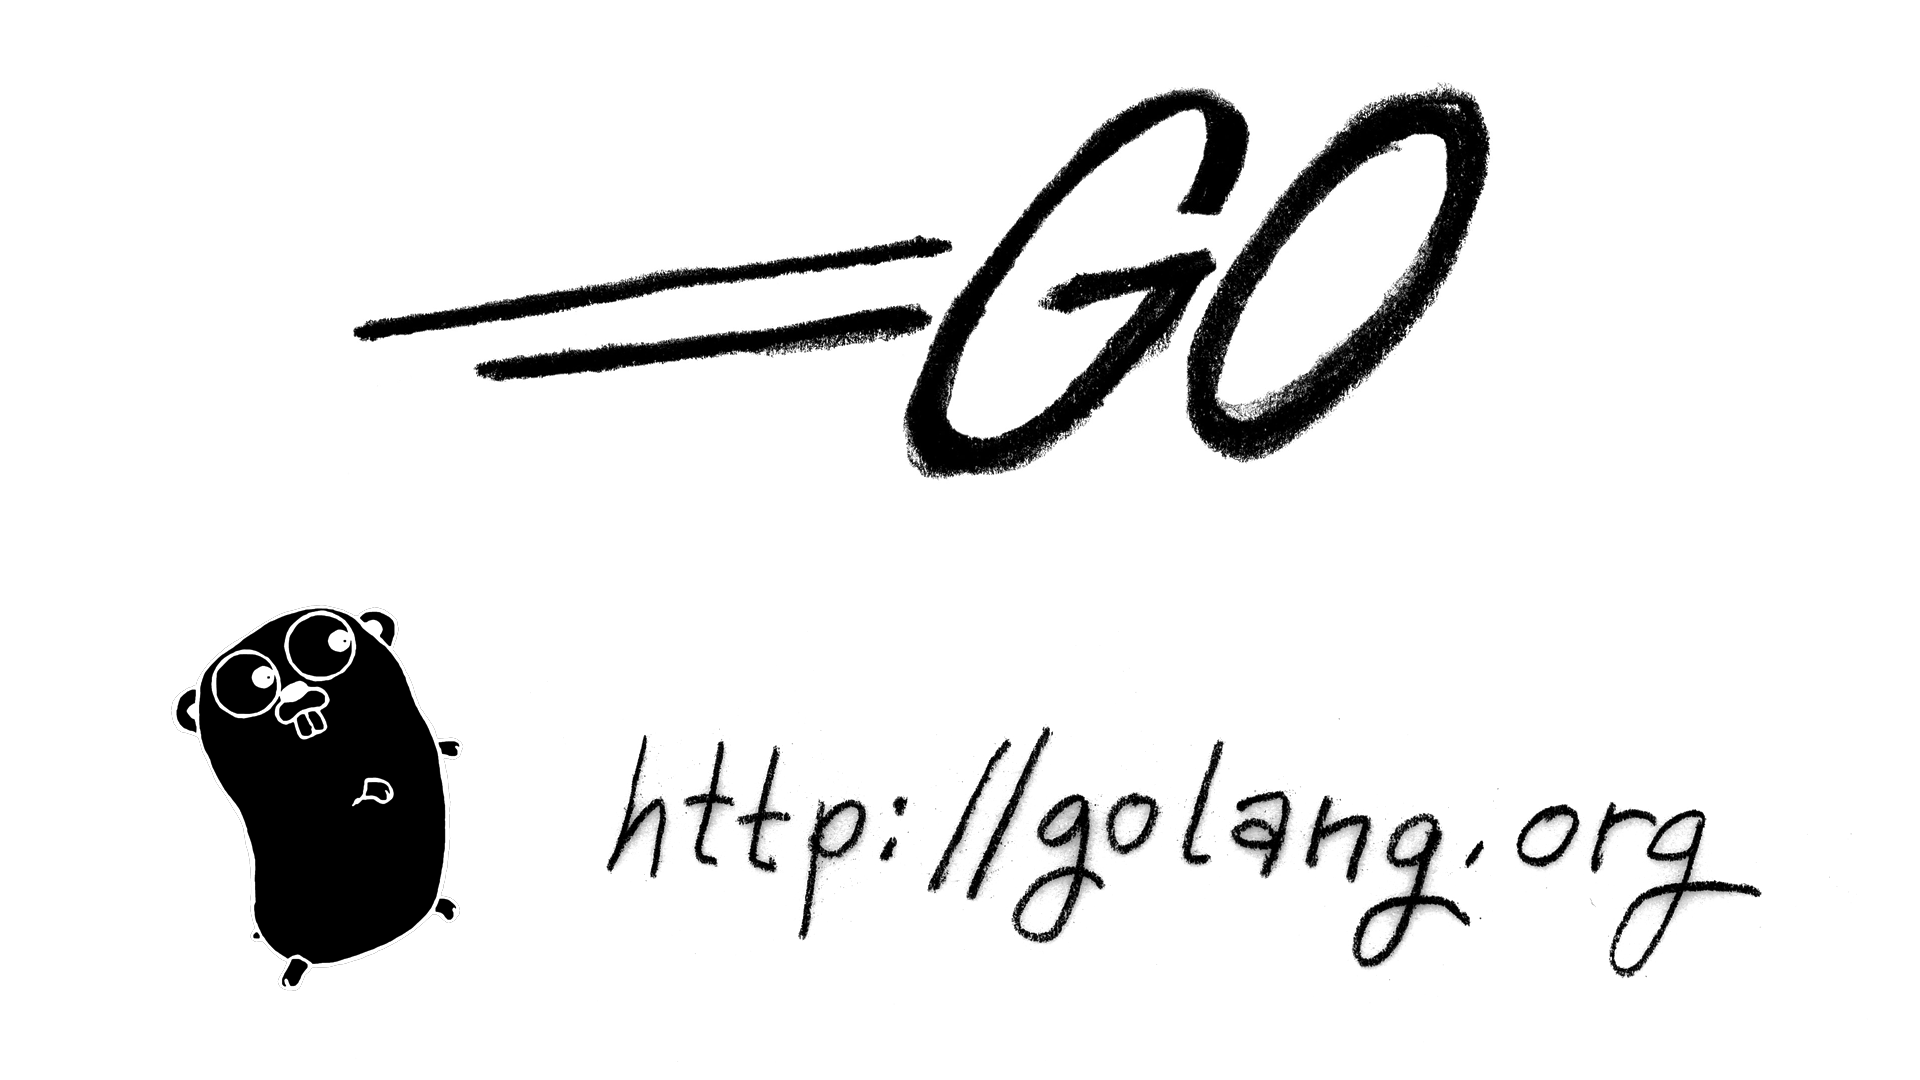
\includegraphics[scale=0.65]{fig/bumper-inverse.png}
\end{center}
\end{figure}
\vspace*{5.0cm}
\begin{minipage}{0.4\textwidth}
\begin{flushleft} \large
\hspace*{2,0cm}\emph{Authors:}\\
\hspace*{2.0cm}Miek Gieben\\
\hspace*{2.0cm}\ \\
\hspace*{2.0cm}\
\vfill
\end{flushleft}
\end{minipage}
%
\begin{minipage}{0.4\textwidth}
\begin{flushright} \large
\emph{Thanks to:} \\
Go authors\\
Google\\
Go Nuts mailing list
\vfill
\end{flushright}
\end{minipage}


\vfill
\begin{center}
\hspace*{2.5cm}THIS IS A WORK IN PROGRESS\newline\newline
    \hspace*{1cm}\CcGroupByNcSa{0.83}{0.95ex}\\[2.5ex]
    \hspace*{1cm}{\tiny\CcNote{\CcLongnameByNcSa}}
\newline\hspace*{1cm}{\tiny Version: \version{} (\today)}
\end{center}
%% End title page %%

\newpage
\pagenumbering{roman}
\tableofcontents
\lstlistoflistings
\listoffigures
\listoftables
\listofex

\clearpage
\thispagestyle{empty}
\begin{figure}[H]
\begin{center}
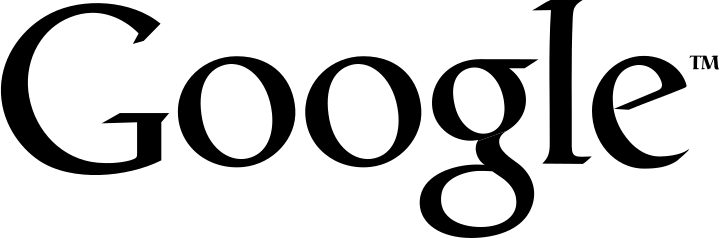
\includegraphics[scale=0.50]{fig/google_logo_black.pdf}
\end{center}
\end{figure}

\begin{center}
\vspace{8.0cm}
Go is \emph{fun}!
\end{center}



\chapter{Introduction}
\label{chap:intro}
\epi{"I am interested in this and hope to do something."}
{\textit{On adding complex numbers to Go}\\ \textsc{KEN THOMPSON}}

\noindent{}What is Go? From the website \cite{go_web}:
\begin{quote}
The Go programming language is an open source project to make
programmers more productive. Go is expressive, concise, clean, and
efficient. Its concurrency mechanisms make it easy to write programs
that get the most out of multi core and networked machines, while its
novel type system enables flexible and modular program construction. Go
compiles quickly to machine code yet has the convenience of garbage
collection and the power of run-time reflection. It's a fast, statically
typed, compiled language that feels like a dynamically typed,
interpreted language.
\end{quote}

Go is a young language, where 
features are still being added or even \emph{removed}. It 
may be possible that some text is outdated when you
read it. 
Some exercise answers may become incorrect as Go continues
to evolve.
We will do our best to keep this document up to 
date with respect to the latest Go release.
An effort has been made to create "future proof" code examples.

The following convention is used throughout this book:
\begin{itemize}
\item Code is displayed in \prog{DejaVu Mono};
\item Keywords are displayed in \key{DejaVu Mono Bold};
\item Comments are displayed in \rem{DejaVu Mono Italic};
\item Extra remarks in the code \coderemark{Are displayed like this};
\item Longer remarks get a number -- \gocircle{1} -- with the explanation following;
\item Line numbers are printed on the right side;
\item Shell examples use a \pr{} as prompt;
\item User entered text in shell examples \texttt{\user{is in bold}}, system responses
are in a \texttt{typewriter font};
\item An emphasized paragraph is indented and has a vertical bar on the
left.
\end{itemize}

\section{Official documentation}
There already is a substantial amount of documentation written about Go.
\gomarginpar{When searching on the internet use the term "golang" instead of plain "go".}
The Go Tutorial \cite{go_tutorial}, and the Effective Go
document \cite{effective_go}. The
website \url{http://golang.org/doc/} is a very good starting point
for reading up on Go\footnote{\url{http://golang.org/doc/} itself is served by 
a Go program called \prog{godoc}.}. Reading these documents is
certainly not required, but is recommended.

Go comes with its own documentation in the form of a Go program called
\prog{godoc}. 
You can use it yourself to look
in the on-line documentation. For
instance, suppose we want to know more about the package \package{hash}.
We would then give the command \prog{godoc hash}.
How to create your own package documentation
is explained in chapter \ref{chap:packages}.

\section{Getting Go}
Ubuntu and Debian both have a Go package in their repositories, look for
the package "golang". But there are still some minor issues being worked
out. For now we will stick to the installation from source.

So we will retrieve the code from the mercurial archive and compile
Go yourself. For other Unix like systems the procedure is the same.
\begin{itemize}
\item First install Mercurial (to get the \prog{hg} command). In
Ubuntu/Debian/Fedora you must install the \prog{mercurial} package;

\item For building Go you need the packages: \prog{bison},
\prog{gcc}, \prog{libc6-dev}, \prog{ed}, \prog{gawk} and \prog{make};

\item Set the environment variable \prog{GOROOT} to the root of your
Go install:
\begin{display}
\pr \user{export GOROOT=~/go}
\end{display}

\item Then retrieve the Go source code:
\begin{display}
\pr \user{hg clone -r release https://go.googlecode.com/hg/ $GOROOT}
\end{display}

\item Set your PATH to so that the Shell can find the Go binaries:
\begin{display}
\pr \user{export PATH=$GOROOT/bin:$PATH}
\end{display}

\item Compile Go
\begin{display}
\pr \user{cd $GOROOT/src}
\pr \user{./all.bash}
\end{display}
\end{itemize}
If all goes well, you should see the following:
\begin{display}
Installed Go for linux/amd64 in /home/go.
Installed commands in /home/go/bin.
The compiler is 6g.
\end{display}
You now have Go installed on your system and you can start playing.

\subsection{Keeping up to date}
New releases are announced on the Go Nuts mailing list \cite{go_nuts}. To update an
existing tree to the latest release, you can run:
\begin{display}
\pr \user{cd $GOROOT}
\pr \user{hg pull}
\pr \user{hg update release}
\pr \user{cd src}
\pr \user{./all.bash}
\end{display}
\noindent{}To see what you are running right now:
\begin{display}
\pr \user{cd $GOROOT}
\pr \user{hg identify}
79997f0e5823 release/release.2010-10-20
\end{display}
\noindent{}That would be release \gorelease{2010-10-20}. The release as 
describe is a "stable" releases,
as opposed to the "weekly" releases that are more volatile. 
If you want to track the weekly releases
instead of the stable ones you can use:
\begin{display}
\pr \user{hg update weekly}
\end{display}
In stead of
\begin{display}
\pr \user{hg update release}
\end{display}

\section{Origins}
Go has it origins in Inferno \cite{inferno} (which in turn was based
upon Plan 9 \cite{plan9}). Inferno included a language called Limbo
\cite{limbo}. Quoting from the Limbo paper:
\begin{quote}
Limbo is a programming language intended for applications running
distributed systems on small computers. It supports modular programming,
strong type checking at compile- and run-time, \emph{inter process
communication over typed channels}, automatic \emph{garbage collection}, and
simple abstract data types. It is designed for safe execution even on
small machines without hardware memory protection.
\end{quote}
One feature of Limbo that is
included in Go is the support for cross compiling.
Another feature Go inherited from Limbo is channels (see chapter
\ref{chap:channels}). Again from the Limbo documentation.
\begin{quote}
[A channel] is a communication mechanism capable of sending and receiving objects of
the specified type to another agent in the system. Channels may be used
to communicate between local processes; using library procedures, they
may be connected to named destinations. In either case send and receive
operations may be directed to them.
\end{quote}
The channels in Go are easier to use than those in Limbo.
If we dig even deeper in the history of Go we also find references
to "Newsqueak" \cite{newsqueak}, which pioneered the use of 
channel communication in a C--like language. Channel
communication isn't unique to these languages, a big non--C--like
language which also uses them is Erlang \cite{erlang}.

\begin{figure}[H]
\caption{Chronology of Go}
\label{fig:chrono-of-go}
\begin{center}
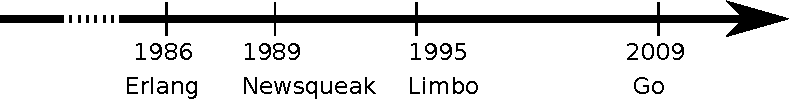
\includegraphics[scale=0.65]{fig/go-history.pdf}
\end{center}
\end{figure}

The whole of idea of using channels to communicate with other processes
is called Communicating Sequential Processes (CSP) and was conceived
by C. A. R. Hoare \cite{hoare}, who incidentally is the same man that
invented QuickSort \cite{quicksort}.

\begin{lbar}[]
Go is the first C--like language that is widely available,
runs on many
different platforms and makes concurrency easy (or easier).
\end{lbar}

\section{Exercises}
\begin{Exercise}[title={文档},difficulty=1]
\label{ex:doc}
\Question
Go 的文档可以通过~\prog{go doc} 程序阅读,它包含在~Go 的发布包中。

\prog{go doc hash} 给出了~\package{hash} 包的信息:
\vskip\baselineskip
\begin{display}
\pr \user{go doc hash}
PACKAGE

package hash

...
...
...

SUBDIRECTORIES

        adler32
        crc32
        crc64
        fnv

\end{display}
\vskip\baselineskip
哪个~\prog{go doc} 的命令可以显示~\package{hash} 包中的~\package{fnv} 文档?

\end{Exercise}

\begin{Answer}
\Question
\package{fnv} 包在~\package{hash} 的\emph{子目录}中,所以只需要 
\quad \texttt{go doc hash/fnv} 即可。


所有的内建函数同样可以通过~\prog{godoc} 程序访问:\prog{go doc builtin}。
\end{Answer}


\cleardoublepage
\section{Answers}
\shipoutAnswer


\chapter{Basics}
\pagenumbering{arabic}
\label{chap:basics}
\epi{"In Go, the code does exactly what it says on the page."}{\textit{Go
Nuts mailing list}\\\textsc{ANDREW GERRAND}}
\noindent{}There are a few things that make Go different from other
languages.
\begin{description}
\item[Clean and Simple]
Go strives to keep things small and beautiful, you should
be able to do a lot in only a few lines of code;
\item[Concurrent]
Go makes it easy to ''fire off'' functions to be
run as \emph{very} lightweight threads. These threads are called
\first{goroutines}{goroutines} \footnote{Yes, that sounds a lot like
\emph{co}routines, but goroutines are slightly different as we will
see in chapter \ref{chap:channels}.} in Go;
%% gofix.go:11: non-declaration statement outside function body
\item[Channels] 
Communication with these goroutines is done
via \first{channels}{channels} \cite{csp, hoare};

\item[Fast]
Compilation is fast and execution is fast. The aim is
to be as fast as C. Compilation time is measured in seconds;

\item[Safe]
Explicit casting and strict rules when converting one type to another.
Go has garbage collection, no more \func{free()} in Go, the language takes care of this;

\item[Standard format]
A Go program can be formatted in (almost) any way the programmers want,
\emph{but} an official format exist. The rule is very simple:
The output of the filter \prog{gofmt} \emph{is the official} endorsed
format.

\item[Postfix types]
Types are given \emph{after} the variable name, thus \prog{var a int},
instead of \prog{int a;} as one would in C;

\item[UTF-8]
UTF-8 is everywhere, in strings
\emph{and} in the program code. Finally you can use \prog{$\Phi$ =
$\Phi$ + 1} in your source code;

\item[Open Source]
The Go license is completely open source, see the file LICENSE in the Go
source code distribution;

\item[Fun]
Programming with Go should be fun!

\end{description}
Erlang \cite{erlang} also shares some
of the features of Go. Notable differences between Erlang
and Go is that Erlang borders on being a functional language,
where Go is an imperative one. And Erlang runs in a virtual
machine, while Go is compiled. Go also has a much more Unix-like
feeling to it.

\section{Hello World}
\label{sec:hello world}
In the Go tutorial, Go is presented to the world in the typical
manner: letting it print "Hello World" (Ken Thompson and
Dennis Ritchie started this when they presented the C language in 
the nineteen seventies). We don't think we can do better, so 
here it is, ''Hello World'' in Go.

\lstinputlisting[numbers=right,label=src:hello,caption=Hello world]{src/helloworld.go}
Lets look at the program line by line.
\showremarks

\section{Compiling and running code}
The Go compiler is named \verb|<number>g|, where the number is 6 for 64 bit
Intel and 8 for 32 bit Intel. The linker has a similar naming scheme:
\verb|<number>l|. In this book we will use \prog{6g} and \prog{6l} for
all the compiles. To compile the code from above, we use:
\begin{display}
\pr \user{6g helloworld.go}
\end{display}

\noindent{}And then we link it with \prog{6l}:
\begin{display}
\pr \user{6l helloworld.6}
\end{display}

\noindent{}And then we run it:
\begin{display}
\pr \user{./6.out}	    \coderemark{The default name for a (64 bit) Go executable (8.out on 32 bits)}
\end{display}
\vspace{-3.0ex}
\texttt{Hello, world; or }%
\begin{math}\kappa\alpha\lambda\eta\mu\acute{\epsilon}\rho\alpha\hspace{1em}\kappa\end{math}%
\'o\begin{math} \sigma\mu\epsilon\end{math}\texttt{; or }\begin{cjk}こんにちは 世界\end{cjk}
\ \newline
\ \newline

\subsection{Using a Makefile}
\label{sec:building a program}
Another, less laborious (once setup), way to build a Go program, is to use a
\file{Makefile}. The following one can be used to build
\prog{helloworld}:
\lstinputlisting[language=make,caption=Makefile for a program,numbers=right,linerange={5,11}]{src/Makefile.prog}
At line 3 you specify the name for your compiled program and on line 5
you enumerate the source files. Now an invocation of \verb|make| is
enough to get your program compiled. Note that Go ships with the variant
of \prog{make}, called \prog{gomake}, which is (currently) a small
wrapper around GNU make. As the build system for Go programs may
change in the future and make \prog{make} go away, we use \prog{gomake}.
Note that this \file{Makefile} creates an executable named
\prog{helloworld}, not \prog{6.out} or \prog{8.out}.

\section{Variables, types and keywords}
\label{sec:vars}
In the next sections we will look at variables, basic types,
keywords and control structures of our new language. 
Go has a C-like feel when it comes to its syntax. 
If you want to put two (or more) statements on one line, they must be
separated with a semicolon (';'). Normally you don't need the semicolon.

Go is different from other languages in that the type of a variable
is specified \emph{after} the variable name. So not: 
\lstinline{int a}, but \lstinline{a int}. When declaring a variable it
is assigned the "natural" null value for the type. This means that after
\lstinline{var a int}, \lstinline{a} has a value of 0. With
\lstinline{var s string}, \lstinline{s} is assigned the zero string,
which is \lstinline{""}. 

Declaring and assigning in Go is a two step process, but they may
be combined. Compare the following pieces of code which have
the same effect. 
\index{variables!declaring}
\index{variables!assigning}

\begin{minipage}{.5\textwidth}
\begin{lstlisting}[linewidth=.5\textwidth,caption={Declaration with =}]
var a int
var b bool
a = 15
b = false
\end{lstlisting}
\hfill
\end{minipage}
\begin{minipage}{.5\textwidth}
\begin{lstlisting}[linewidth=.5\textwidth,caption={Declaration with :=}]
a := 15
b := false
\end{lstlisting}
\ \\
\ \\
\hfill
\end{minipage}

On the left we use the
\key{var} keyword to declare a variable and \emph{then} assign a value to
it. The code on the right uses \mbox{\key{:=}{ }} to do this in one
step (this form may only be used \emph{inside} functions).
In that case the variable
type is \emph{deduced} from the value. A value of 15 indicates an \type{int},
a value of \texttt{false} tells Go that the type should be \type{bool}. 
Multiple \key{var} declarations may also be grouped, \key{const}
and \key{import} also allow this. Note the use of parentheses:
\begin{lstlisting}
var (
    x int
    b bool
)
\end{lstlisting}
Multiple variables of the same type can also be declared on a
single line: \lstinline{var x, y int}, makes \var{x} and \var{y} both
\type{int} variables. You can also make use of \first{parallel
assignment}{parallel assignment}:
\begin{lstlisting}
a, b := 20, 16
\end{lstlisting}
Which makes \var{a} and \var{b} both integer variables and assigns
20 to \var{a} and 16 to \var{b}.

A special name for a variable is \var{\textbf{\_}} \index{variables!\_}
(underscore) \index{variables!underscore}. Any value
assigned to it, is discarded. In this example we only assign the integer
value of 35 to \var{b} and discard the value 34.
\begin{lstlisting}
_, b := 34, 35
\end{lstlisting}
Declared, but otherwise unused variables are a compiler error in Go. The
following code generates this error:
\error{i declared and not used}

\begin{lstlisting}
package main
func main() { 
    var i int
}
\end{lstlisting}

\subsection{Boolean types}
A boolean type represents the set of boolean truth values denoted by the
predeclared constants \emph{true} and \emph{false}. The boolean type is \type{bool}.

\subsection{Numerical types}
Go has the well known types such as \lstinline{int}, this type
has the appropriate length for your machine. 
Meaning that on a 32 bits machine they are 32 bits, and on
a 64 bits machine they are 64 bits. Note: an \lstinline{int} is
either 32 or 64 bits, no other values are defined. Same goes 
for \lstinline{uint}.

If you want to be explicit about the length you can have
that too with \lstinline{int32}, or \lstinline{uint32}. The full
list for (signed and unsigned) integers is
\type{int8}, \type{int16}, \type{int32}, \type{int64} and
\type{byte}, \type{uint8}, \type{uint16}, \type{uint32}, \type{uint64}.
With \lstinline{byte} being an
alias for \lstinline{uint8}. For floating point values there is
\lstinline{float32} and \lstinline{float64} (there is no \lstinline{float} type). 
A 64 bit integer or floating point value is \emph{always} 64 bit, also on 32 bit
architectures.

Note however
that these types are all distinct and assigning variables which mix
these types is a compiler error, like in the following code:
\lstinputlisting[numbers=right,label=src:types,caption=Familiar types are still distinct]{src/types.go}
Gives the error on the assignment on line 7:

\noindent\error{types.go:7: cannot use a + a (type int)  as type int32 in assignment}

The assigned values may be denoted using octal, hexadecimal or the scientific notation:
\lstinline{077}, \lstinline{0xFF}, \lstinline{1e3} or
\mbox{\lstinline{6.022e23}} are all valid.

\subsection{Constants}
\label{sec:constants}
Constants in Go are just that --- constant. They are created at compile
time, and can only be numbers, strings or booleans;
\lstinline{const x = 42} makes \var{x} a constant. You can use
\first{\key{iota}}{keyword!iota} \footnote{The word [iota] is used in a common English phrase,
'not one iota', meaning 'not the slightest difference', in reference to
a phrase in the New Testament: "\emph{until heaven and earth pass away, not an
iota, not a dot, will pass from the Law}." \cite{iota}}
to enumerate values.
\begin{lstlisting}
const (
	a = iota
	b = iota 
)
\end{lstlisting}
The first use of \key{iota} will yield 0, so \var{a} is equal to 0, whenever
\key{iota} is used again on a new line its value is incremented with 1, so \var{b}
has a value of 1.

You can even do the following, let Go repeat the use of \key{= iota}:
\begin{lstlisting}
const (
	a = iota
	b	    |\coderemark{Implicitly \texttt{b = iota}}|
)
\end{lstlisting}
You may also explicitly type a constant, if you need that:
\begin{lstlisting}
const (
	a = 0           |\coderemark{Is an \key{int} now}|
	b string = "0" 
)
\end{lstlisting}

\subsection{Strings}
An important other built in type is \lstinline{string}. Assigning a
string is as simple as:
\begin{lstlisting}
s := "Hello World!"
\end{lstlisting}
Strings in Go are a sequence of UTF-8 characters enclosed in double
quotes ("). If you use the single quote (') you mean one character
(encoded in UTF-8) --- which is \emph{not} a \lstinline{string} in Go.

Once assigned to a variable the string can not be changed anymore: strings in Go are
immutable. For
people coming from C, the following is not legal in Go:
\begin{lstlisting}
var s string = "hello"
s[0] = 'c'  |\coderemark{Change first char. to 'c', this is an error}|
\end{lstlisting}
To do this in Go you will need the following:
\begin{lstlisting}
s := "hello"
c := []byte(s)	    |\longremark{Convert \var{s} to an array of bytes, see %
chapter \ref{chap:beyond} section "\titleref{sec:conversions}" on %
page \pageref{sec:conversions};}|
c[0] = 'c'	    |\longremark{Change the first element of this %
array;}|
s2 := string(c)     |\longremark{Create a \emph{new} %
string \var{s2} with the alteration;}|
fmt.Printf("%s\n", s2) |\longremark{print the string with \func{fmt.Printf}.}|
\end{lstlisting}
\showremarks

\begin{lbar}[Multi-line strings]
Due to the insertion of semicolons (see \cite{effective_go} section
"Semicolons"), you need to be careful with using multi line strings. If
you write:
\begin{lstlisting}
s := "Starting part"
    + "Ending part"
\end{lstlisting}
This is transformed into:
\begin{lstlisting}
s := "Starting part";
    + "Ending part";
\end{lstlisting}
Which is not valid syntax, you need to write:
\begin{lstlisting}
s := "Starting part" +
     "Ending part"
\end{lstlisting}
Then Go will not insert the semicolons in the wrong places. Another way
would be to use \emph{raw} string literals\index{string literal!raw} by using back quotes: \key{`}:
\begin{lstlisting}
s := `Starting part
     Ending part`
\end{lstlisting}
Be aware that in this last example \var{s} now also contains the newline.
Unlike \emph{interpreted} string literals \index{string literal!interpreted} a raw string literal's value
is composed of the \emph{uninterpreted} characters between the quotes.
\end{lbar}
\subsection{Complex numbers}
Go has native support for complex numbers. If you 
use them you need a variable of the type \lstinline{complex128} (64
bit imaginary part). If you
want something smaller there is \lstinline{complex64} -- for a 32 bits
imaginary part.
Complex numbers are written as
\var{re + im$i$}, where \var{re} is the real part,
\var{im} is the imaginary part and $i$ is the literal '$i$' ($\sqrt{-1}$).
An example of using complex numbers:

\lstinline{var c complex64 = 5+5i; fmt.Printf("Value is: %v", c)}\newline
will print: \lstinline{(5+5i)}

\subsection{Error}
Any non-trivial program will need errors sooner or later. Because of this
Go has a builtin type specially for errors


\section{Operators and built-in functions}
Go supports the normal set of numerical operations,
table \ref{tab:op-precedence}
lists the current ones and their relative precedence. They
all associate from left to right.

\begin{table}[H]
\begin{center}
\caption{Operator precedence}
\label{tab:op-precedence}
\begin{tabular}{ll}
\textbf{precedence} & \textbf{operator(s)} \\ \hline
highest   &	\verb!*  /  %  <<  >>  &  &^!		\\
    &	\verb!+  -  | ^!			\\
    &	\verb+==  !=  <  <=  >  >=+		\\
    &	\verb!<-!				\\
    &	\verb!&&!				\\
lowest    &	\verb!||!				\\
\end{tabular}

\end{center}
\end{table}
\verb|+ - * /| and \verb|%| all do what you would expect,
\verb!& | ^!
and \verb!&^! are bit operators for
\first{\key{bitwise and}}{operator!bitwise!and}, 
\first{\key{bitwise or}}{operator!bitwise!or}, \first{\key{bitwise xor}}{operator!bit
wise xor} and \first{\key{bit clear}}{operator!bitwise!clear} respectively.
The \verb|&&| and \verb/||/ operators are 
logical \first{\key{and}}{operator!and} and
logical \first{\key{or}}{operator!or}. Not listed in the table
is the logical \first{\key{not}}{operator!not}: \verb/!/ .

Although Go does not support operator overloading (or method
overloading for that matter), some of the built-in
operators \emph{are} overloaded. For instance \texttt{+} can be used for integers,
floats, complex numbers and strings (adding strings is concatenating
them). 

\section{Go keywords}
\begin{table}[H]
\begin{center}
\caption{Keywords in Go}
\label{tab:keywords}
%%%%%%%%%%%%%%%%%%%%%%%%%%%%%%%%%%%%%%%%%%%%%%%%%%%%%%%%%%%%%%%%%%%%%%
%%                                                                  %%
%%  This is a LaTeX2e table fragment exported from Gnumeric.        %%
%%                                                                  %%
%%%%%%%%%%%%%%%%%%%%%%%%%%%%%%%%%%%%%%%%%%%%%%%%%%%%%%%%%%%%%%%%%%%%%%
\begin{tabular}{lllll}
\key{break}	&\key{default}          &\key{for}	&\key{import}    &\key{return}\\
\key{case}	&\key{defer}            &\key{func}	&\key{interface}          &\key{select}\\
\key{chan}	&\key{delete}           &\key{go}	&\key{map}      &\key{struct}\\
\key{const}	&\key{else}    	    &\key{goto}	&\key{package}        &\key{switch}\\
\key{continue}	&\key{fallthrough}      &\key{if}	&\key{range}       &\key{type}\\
               &                       &               &                   &\key{var}\\
\end{tabular}

\end{center}
\end{table}
Table \ref{tab:keywords} lists all the keywords in Go. 
In the following paragraphs and chapters we will cover them. Some
of these we have seen already.
\begin{itemize}
\item For \key{var} and \key{const} see section "\titleref{sec:vars}" on 
page \pageref{sec:vars};
\item \key{package} and \key{import} are briefly touched upon in section "\titleref{sec:hello world}". 
In chapter \ref{chap:packages} they are documented in more detail.
\end{itemize}
Others deserve more text and have their own chapter/section:
\begin{itemize}
\item \key{func} is used to declare functions and methods;
\item \key{return} is used to return from functions, for both \key{func}
and \key{return} see chapter \ref{chap:functions} for the details;
\item \key{go} is used for concurrency (chapter \ref{chap:channels});
\item \key{select} used to choose from different types of communication, see chapter \ref{chap:channels};
\item \key{interface} see chapter \ref{chap:interfaces};
\item \key{struct} is used for abstract data types, see chapter \ref{chap:beyond};
\item \key{type} also see chapter \ref{chap:beyond}.
\end{itemize}

\section{Control structures}
There are only a few control structures in 
Go \footnote{This section is copied from \cite{effective_go}.}.
For instance there is no do or while loop, only a 
\key{for}. There is a (flexible) \key{switch} statement and \key{if} and
\key{switch} accept an
optional initialization statement like that of \key{for}. There also is
something called a type switch and a multiway communications
multiplexer, \key{select} (see chapter \ref{chap:channels}). The syntax is 
different (from that in C): parentheses
are not required and the body must \emph{always} be brace-delimited.

\subsection{If}
In Go an \first{\key{if}}{keyword!if} looks like this:
\begin{lstlisting}
if x > 0 {	|\coderemark{\{ is mandatory}|
    return y
} else {
    return x
}
\end{lstlisting}
Mandatory braces encourage writing simple \key{if} statements on multiple
lines. It is good style to do so anyway, especially when the body
contains a control statement such as a
\first{\key{return}}{keyword!return} or
\first{\key{break}}{keyword!break}.

Since \key{if} and \key{switch} accept an initialization statement, it's common to
see one used to set up a (local) variable.
\begin{lstlisting}
if err := file.Chmod(0664); err != nil {  |\coderemark{\texttt{nil} is %
like C's NULL}|
    log.Stderr(err) |\coderemark{Scope of \var{err} is limited to %
\key{if}'s body}|
    return err
}
\end{lstlisting}
You can use the logical operators (see table \ref{tab:op-precedence}) as
you would normally do:
\begin{lstlisting}
if true && true  {
    println("true")
}
if ! false {
    println("true")
}
\end{lstlisting}

In the Go libraries, you will find that when an \key{if} statement doesn't flow
into the next statement -- that is, the body ends in \key{break},
\key{continue}, \key{goto},
or \key{return} -- the unnecessary \first{\key{else}}{keyword!else} is omitted.

\begin{lstlisting}
f, err := os.Open(name, os.O_RDONLY, 0)
if err != nil {
    return err
}
doSomething(f)
\end{lstlisting}
This is a example of a common situation where code must analyze a
sequence of error possibilities. The code reads well if the successful
flow of control runs down the page, eliminating error cases as they
arise. Since error cases tend to end in \key{return} statements, the resulting
code needs no \key{else} statements.
\begin{lstlisting}
f, err := os.Open(name, os.O_RDONLY, 0)
if err != nil {
    return err
}
d, err := f.Stat()
if err != nil {
    return err
}
doSomething(f, d)
\end{lstlisting}
Syntax wise the following is illegal in Go:
\begin{lstlisting}
if err != nil
{		    |\coderemark{Must be on the same line as the if}|
    return err
}
\end{lstlisting}
See \cite{effective_go} section "Semicolons" for the deeper reasons
behind this.

\begin{lbar}[Ending with \key{if-then-else}]
Note that if you end a function like this:
\begin{lstlisting}
if err != nil {
    return err
} else {
    return nil
}
\end{lstlisting}
It will not compile. This is a bug in the Go compiler. See
\cite{go_issue_65} for an extended problem description and
hopefully a fix.
\end{lbar}

\subsection{Goto}
Go has a \first{\key{goto}}{keyword!goto} statement --- use it wisely. With \key{goto}
you jump to a \index{label} label which must be defined within the current function.
For instance a loop in disguise:
\begin{lstlisting}
func myfunc() {
        i := 0                                                                                      
Here:	   |\coderemark{First word on a line ending with a colon is a label}|
        println(i)
        i++ 
        goto Here |\coderemark{Jump}|
}
\end{lstlisting}
The name of the label is case sensitive.

\subsection{For}
\label{sec:for}
The Go \first{\key{for}}{keyword!for} loop has three forms, only one of
which has semicolons.
\begin{lstlisting}
for init; condition; post { } |\coderemark{Like a C \key{for}}|

for condition { }             |\coderemark{Like a while}|

for { }                       |\coderemark{ Like a C \key{for(;;)} (endless loop)}|
\end{lstlisting}
Short declarations make it easy to declare the index variable right in the loop.
\begin{lstlisting}
sum := 0
for i := 0; i < 10; i++ {
    sum += i	|\coderemark{Short for sum = sum + i}|
}   |\coderemark{\var{i} ceases to exist \emph{after} the loop}|
\end{lstlisting}
Finally, since Go has no comma operator and ++ and - - are statements not
expressions, if you want to run multiple variables in a \key{for} you should
use \first{parallel assignment}{parallel assignment}.
\begin{lstlisting}
// Reverse a
for i, j := 0, len(a)-1; i < j; i, j = i+1, j-1 { |\coderemark{Parallel assignment}|
    a[i], a[j] = a[j], a[i] |\coderemark{Here too}|
}
\end{lstlisting}

\subsection{Break and continue}
With \first{\key{break}}{keyword!break} you can quit loops early.  By itself, \key{break} breaks
the current loop.
\begin{lstlisting}
for i := 0; i < 10; i++ {
    if i > 5 {
	break |\coderemark{Stop this loop, making it only print 0 to 5}|
    }
    println(i)
}
\end{lstlisting}
With loops within loops you can specify a label after \key{break}.
Making the label identify \emph{which} loop to stop:
\begin{lstlisting}
J:  for j := 0; j < 5; j++ {
	for i := 0; i < 10; i++ {
	    if i > 5 { 
		break J	|\coderemark{Now it breaks the \var{j}-loop, not the \var{i} one}|
	    }
	    println(i)
	}
    } 
\end{lstlisting}

With \first{\key{continue}}{keyword!continue} you begin the next iteration of the
loop, skipping any remaining code. In the same way as \key{break},
\key{continue} also accepts a label. The following prints 0 to 5.
\begin{lstlisting}
for i := 0; i < 10; i++ {
    if i > 5 {
	continue |\coderemark{Skip any remaining code}|
    }
    println(i)
}
\end{lstlisting}

\subsection{Range}
The keyword \first{\key{range}}{keyword!range} can be used for loops. It
can loop over slices, arrays, strings, maps and channels (see chapter
\ref{chap:channels}). \key{range} is
an iterator that, when called, returns a key-value pair from the thing it
loops over. Depending on what that is, \key{range} returns
different things.

When looping over a slice or array \key{range} returns the index in the
slice as the key and value belonging to that index.
Consider this code: \index{keyword!range!on slices}
\begin{lstlisting}
list := []string{"a", "b", "c", "d", "e", "f"}     |\longremark{Create a %
slice (see "\titleref{sec:arrays}" on page \pageref{sec:arrays})) of strings.}|
for k, v := range list {	|\longremark{Use \key{range} to loop over them.%
With each iteration \key{range} will return the index as \type{int} and %
the key as a \type{string}, starting with 0 and "a".}|
    // do what you want with k and v \longremark{\var{k} will have the value 0\ldots5, and %
\var{v} will loop through "a"\ldots"f".}
}
\end{lstlisting}
\showremarks

You can also use \key{range} on strings directly. Then it
will break out the individual Unicode characters 
\footnote{In the UTF-8 world characters are sometimes called \first{runes}{runes}. 
Mostly, when people talk about
characters, they mean 8 bit characters. As UTF-8 characters may be up to 32 bits the word
rune is used.} and their start position, by parsing the UTF-8.
The loop: \index{keyword!range!on maps}
\begin{lstlisting}
for pos, char := range "a|$\Phi{}$|x" {
    fmt.Printf("character '%c' starts at byte position %d\n", char, pos)
}
\end{lstlisting}
prints
\begin{display}
character 'a' starts at byte position 0
character '\begin{math}\Phi\end{math}' starts at byte position 1
character 'x' starts at byte position 3 \coderemark{\begin{math}\Phi\end{math} took 2 bytes}
\end{display}

\subsection{Switch}
Go's \first{\key{switch}}{keyword!switch} is very flexible. The expressions need
not be
constants or even integers, the cases are evaluated top to bottom until
a match is found, and if the \key{switch} has no expression it switches on
\type{true}. It's therefore possible -- and idiomatic -- to write an
\key{if-else-if-else} chain as a \key{switch}.
\begin{lstlisting}
func unhex(c byte) byte {
    switch {
    case '0' <= c && c <= '9':
        return c - '0'
    case 'a' <= c && c <= 'f':
        return c - 'a' + 10
    case 'A' <= c && c <= 'F':
        return c - 'A' + 10
    }
    return 0
}
\end{lstlisting}
There is no automatic fall through, you can however use
\first{\key{fallthrough}}{keyword!fallthrough} to do just that.
Without \key{fallthrough}:
\begin{lstlisting}
switch i {
    case 0:  // empty case body
    case 1:
	f()  // f is not called when i == 0!
}
\end{lstlisting}
And with:
\begin{lstlisting}
switch i {
    case 0:  fallthrough
    case 1:
	f()  // f is called when i == 0!
}
\end{lstlisting}
With \first{\key{default}}{keyword!default} you can specify an action
when none of the other cases match.
\begin{lstlisting}
switch i {
    case 0:  
    case 1:
	f()
    default:	
	g()	// called when i is not 0 or 1
}
\end{lstlisting}
Cases can be presented in comma-separated lists.
\begin{lstlisting}
func shouldEscape(c byte) bool {
    switch c {
    case ' ', '?', '&', '=', '#', '+': |\coderemark{, as "or"}|
        return true
    }
    return false
}
\end{lstlisting}
Here's a comparison routine for byte arrays that uses two \key{switch} statements:
\begin{lstlisting}
// Compare returns an integer comparing the two byte arrays
// lexicographically.
// The result will be 0 if a == b, -1 if a < b, and +1 if a > b
func Compare(a, b []byte) int {
    for i := 0; i < len(a) && i < len(b); i++ {
        switch {
        case a[i] > b[i]:
            return 1
        case a[i] < b[i]:
            return -1
        }
    }
    // String are equal except for possible tail
    switch {
    case len(a) < len(b):
        return -1
    case len(a) > len(b):
        return 1
    }
    return 0	// Strings are equal
}
\end{lstlisting}

\section{Built-in functions}
A small number of functions are predefined, meaning 
you \emph{don't} have to include any package to get
access to them. Table \ref{tab:predef-functions} lists them all.

\begin{table}[H]
\begin{center}
\caption{Pre--defined functions in Go}
\label{tab:predef-functions}
\begin{tabular}{lllll}
\key{close}	&\key{new}	&\key{panic}	&\key{complex} \\
\key{delete}   &\key{make}     &\key{recover}  &\key{real} \\
\key{len}	&\key{append}	&\key{print}	&\key{imag}  \\
\key{cap}	&\key{copy}	&\key{println}	&\\
\end{tabular}

\end{center}
\end{table}

These built-in functions are documented in the \package{builtin} \index{package!builtin}
pseudo package that is included in recent Go releases.

\paragraph{\func{close}} is used in
channel communication. It closes a channels, see chapter \ref{chap:channels}
for more on this.
\index{built-in!close}

\paragraph{\func{delete}} is used for deleting entries in maps.
\index{built-in!delete}

\paragraph{\func{len} and \func{cap}} are used on a number of different
types, \func{len} is
used for returning the length of strings and the length of slices and
arrays. See section "\titleref{sec:arrays}" for the details of slices and
arrays and the function
\func{cap}.\index{built-in!len}\index{built-in!cap}

\paragraph{\func{new}} is used for allocating memory for user defined
data types. See section "\titleref{sec:allocation with new}" on page
\pageref{sec:allocation with new}.
\index{built-in!new}

\paragraph{\func{make}} is used for allocating memory for built-in
types (maps, slices and channels). See section 
"\titleref{sec:allocation with make}" on page
\pageref{sec:allocation with make}.
\index{built-in!make}

\paragraph{\func{copy}} is used for copying slices. \func{append} is 
for concatenating slices. See section "\titleref{sec:slices}" in this
chapter.
\index{built-in!copy}
\index{built-in!append}

\paragraph{\func{panic} and \func{recover}} are used for an 
\emph{exception} mechanism. See the section "\titleref{sec:panic}" on 
page \pageref{sec:panic} for more.
\index{built-in!panic}
\index{built-in!recover}

\paragraph{\func{print} and \func{println}} are low level printing
functions that can be used without reverting to the
\package{fmt}\index{package!fmt}
package. These are mainly used for debugging.
\index{built-in!print}\index{built-in!println}

\paragraph{\func{complex}, \func{real} and \func{imag}} all deal with
\first{complex numbers}{complex numbers}. Other than the simple example
we gave, we will not further explain complex numbers.
\index{built-in!complex}
\index{built-in!real}
\index{built-in!imag}


\section{Arrays, slices and maps}
\label{sec:arrays}
Storing multiple values in a list can be done by utilizing arrays, or
their more flexible cousin: slices. A dictionary or hash type is also
available, it is called a \type{map} in Go.

\subsection{Arrays}
An array is defined by: \verb|[n]<type>|, where $n$ is the length
of the array and \verb|<type>| is the stuff you want to store.
Assigning, or indexing an element in the array is done with square
brackets:
\begin{lstlisting}
var arr [10]int
arr[0] = 42
arr[1] = 13
fmt.Printf("The first element is %d\n", arr[0])
\end{lstlisting}
Array types like \lstinline{var arr = [10]int} have a fixed size. The
size is \emph{part} of the type.
They can't grow, because then they would have a different type. Also arrays
are values: Assigning one array to another \emph{copies} all the elements.
In particular, if you pass an array to a function, it will receive a
copy of the array, not a pointer to it. 

\index{array!multidimensional}
To declare an array you can use the following: \lstinline{var a [3]int},
to initialize it to something else than zero, use a 
\first{composite literal}{literal!composite}: \lstinline|a := [3]int{1, 2, 3}| and
this can be shortened to \lstinline|a := [...]int{1, 2, 3}|, where Go counts
the elements automatically. \gomarginpar{A composite literal allows you
to assign a value directly to an array, slice or map.

See the section "\titleref{sec:constructors and composite literals}" on
page \pageref{sec:constructors and composite literals} for more.}
Note that all fields must be specified.  So if you are using multidimensional
arrays you have to do quite some typing:
\begin{lstlisting}
a := [2][2]int{ [2]int{1,2}, [2]int{3,4} }
\end{lstlisting}
Which is the same as:
\begin{lstlisting}
a := [2][2]int{ [...]int{1,2}, [...]int{3,4} }
\end{lstlisting}
When declaring arrays you \emph{always} have to type something in
between the square brackets, either a number or three dots (\verb|...|)
when using a composite literal. 
\gomarginpar{Go release \gorelease{2010-10-27} \cite{go_release_hist}.} 
Since release \gorelease{2010-10-27} this syntax was further simplified.
From the release notes:
\begin{quote}
The syntax for arrays, slices, and maps of composite literals has been
simplified. Within a composite literal of array, slice, or map type, elements
that are themselves composite literals may elide the type if it is identical to
the outer literal's element type. 
\end{quote}
This means our example can become:
\begin{lstlisting}
a := [2][2]int{ {1,2}, {3,4} }
\end{lstlisting}

\subsection{Slices}
\label{sec:slices}
\todo{Add push/pop to this section as container/vector will be depricated.}
A slice is similar to an array, but it can grow when new elements
are added.
A slice always refers to an underlying array. What makes slices different
from
arrays is that a slice is a pointer \emph{to} an array;
slices are \first{reference types}{reference types}, 
\gomarginpar{Reference types are created with \lstinline{make}.}
which means that if you assign one slice to
another, both refer to the same underlying array. For instance, if a
function takes a slice argument, changes it makes to the elements of the
slice will be visible to the caller, analogous to passing a pointer to
the underlying array. With:
\begin{lstlisting}
sl := make([]int, 10)
\end{lstlisting}
you create a slice which can hold ten elements. Note that the
underlying array isn't specified.
A slice is always coupled to an array that has
a fixed size. For slices we define a \first{capacity}{slice!capacity} and a
\first{length}{slice!length}. \index{array!length}\index{array!capacity}
Figure \ref{fig:array-vs-slice} depicts the following Go code.
First we create an array of $m$ elements of the type \lstinline{int}:
\lstinline{var array[m]int}\newline
Next, we create a slice from this array:
\lstinline{slice := array[0:n]}\newline
And now we have:
\begin{itemize}
\item{\lstinline{len(slice) == n == cap(slice) == n}{} ;}
\item{\lstinline{len(array) == cap(array) == m}{} .}
\end{itemize}
\begin{figure}[H]
\caption{Array versus slice}
\label{fig:array-vs-slice}
\begin{center}
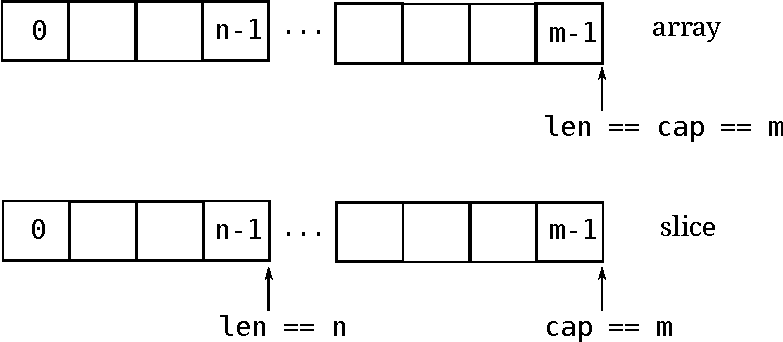
\includegraphics[scale=0.65]{fig/array-vs-slice.pdf}
\end{center}
\end{figure}

Given an array, or another slice, a new slice is created via
\lstinline{a[I:J]}. This creates a new slice which refers to 
\lstinline{a}, starts at index \var{I}, and ends
before index \var{J}. It has length \lstinline{J - I}.

\begin{lstlisting}
// array[n:m], create a slice from array with elements n to m-1
a := [...]int{1, 2, 3, 4, 5} |\longremark{Define an array with 5 %
elements, from index 0 to 4;}|
s1 := a[2:4] |\longremark{Create a slice with the elements from index 2 %
to 3, this contains: \texttt{3, 4};}|
s2 := a[1:5] |\longremark{Create a slice with the elements from index 1 %
to 4, contains: \texttt{2, 3, 4, 5};}|
s3 := a[:]   |\longremark{Create a slice with all the elements of the %
array in it. This is a shorthand for: \texttt{a[0:len(a)]};}|
s4 := a[:4]  |\longremark{Create a slice with the elements from index %
0 to 3, this is thus short for: \texttt{a[0:4]}, and yields: \texttt{1, 2, %
3, 4};}|
s5 := s2[:]  |\longremark{Create a slice from the slice \var{s2}, note that %
\texttt{s5} still refers to the array \texttt{a}.}|
\end{lstlisting}
\showremarks

In the code listed in \ref{src:arrays} we dare to do the impossible on
line 8 and try to allocate something
beyond the capacity (maximum length of the underlying array) and
we are greeted with a \emph{runtime} error.
\lstinputlisting[numbers=right,label=src:arrays,caption=Arrays and slices]{src/array-and-slices.go}
If you want to extend a slice, there are a couple of built-in functions
that make life easier:
\lstinline{append} and \lstinline{copy}. From \cite{go_spec}:
\begin{quote}
The function \lstinline{append} appends zero or more values \lstinline{x} to a
slice \lstinline{s} and returns the resulting slice, with the same type as
\lstinline{s}.
If the capacity of \lstinline{s} is not large enough to fit the additional values,
\lstinline{append} allocates a new, sufficiently large slice that fits both the
existing slice elements and the additional values. Thus, the returned
slice may refer to a different underlying array.
\end{quote}
\index{built-in!append}
\begin{lstlisting}
s0 := []int{0, 0}
s1 := append(s0, 2)       |\longremark{append a single element, \texttt{s1 == []int\{0, 0, 2\}};}|
s2 := append(s1, 3, 5, 7) |\longremark{append multiple elements, %% 
\texttt{s2 == []int\{0, 0, 2, 3, 5, 7\}};}|
s3 := append(s2, s0...)   |\longremark{append a slice, \texttt{s3 == []int\{0, 0, 2, 3, 5, 7, 0, 0\}}. %%
Note the three dots!}|
\end{lstlisting}
\showremarks
And
\begin{quote}
The function \lstinline{copy} copies slice elements from a source
\lstinline{src} to a
destination \lstinline{dst} and returns the number of elements copied. Source and
destination may overlap. The number of arguments
copied is the minimum of \lstinline{len(src)} and
\mbox{\lstinline{len(dst)}}.
\end{quote}
\index{built-in!copy}
\begin{lstlisting}
var a = [...]int{0, 1, 2, 3, 4, 5, 6, 7}
var s = make([]int, 6)
n1 := copy(s, a[0:])    |\coderemark{\texttt{n1 == 6, s == []int\{0, 1, 2, 3, 4, 5\}}}|
n2 := copy(s, s[2:])    |\coderemark{\texttt{n2 == 4, s == []int\{2, 3, 4, 5, 4, 5\}}}|
\end{lstlisting}

\subsection{Maps}
\label{sec:maps}
Many other languages have a similar type built-in, Perl has hashes,
Python has its dictionaries and C++ also has maps (as part of its library) for instance. 
In Go we have the
\first{\key{map}}{keyword!map} type. A \type{map} can be thought of as an array indexed by
strings (in its most simple form).
In the following listing we define a \type{map} which converts from a
\lstinline{string} (month abbreviation) to an \lstinline{int} -- the number of days in that month. 
The generic way to define a map is with: \verb|map[<from type>]<to type>|

\begin{lstlisting}
monthdays := map[string]int{
	"Jan": 31, "Feb": 28, "Mar": 31, 
	"Apr": 30, "May": 31, "Jun": 30, 
	"Jul": 31, "Aug": 31, "Sep": 30, 
	"Oct": 31, "Nov": 30, "Dec": 31, |\coderemark{The comma here is required}|
}		    
\end{lstlisting}
Note to use \lstinline{make} when only declaring a \lstinline{map}:
\lstinline|monthdays := make(map[string]int)|

For indexing (searching) in the map, we use square brackets. For example,
suppose we want to print the
number of days in December: \lstinline{fmt.Printf("%d\n", monthdays["Dec"])}\newline
If you are looping over an array, slice, string, or map a
\first{\key{range}}{keyword!range}
clause help you again, which returns the key and corresponding value
with each invocation.\index{keyword!range!on maps}
\begin{lstlisting}
year := 0
for _, days := range monthdays {    |\coderemark{Key is not used, hence \texttt{\_, days}}|
    year += days
}
fmt.Printf("Numbers of days in a year: %d\n", year)
\end{lstlisting}
Adding elements to the \type{map} \index{keyword!map!add elements} would be done as:
\begin{lstlisting}
monthdays["Undecim"] = 30	|\coderemark{Add a month}|
monthdays["Feb"]     = 29	|\coderemark{Overwrite entry - for leap years}|
\end{lstlisting}
To test for existence \index{keyword!map!existence}, you would use the
following\cite{go_course_day2}:
\begin{lstlisting}
var value int
var present bool

value, present = monthdays["Jan"] |\coderemark{If exist, \texttt{present} has the value \key{true}}|
                                  |\coderemark{Or better and more Go like}|
v, ok := monthdays["Jan"]	  |\coderemark{Hence, the "comma ok" form}|
\end{lstlisting}
And finally you can remove elements \index{keyword!map!remove elements} from the \type{map}:
\begin{lstlisting}
delete monthdays["Mar"]           |\coderemark{Deletes "Mar", always rainy anyway}|
\end{lstlisting}
In general the syntax \lstinline{delete(m, x)} will delete the map entry
retrieved by the expression \lstinline{m[x]}.

\section{Exercises}
\begin{Exercise}[title={For-loop},difficulty=1]
\label{ex:for-loop}
\Question \label{ex:for-loop q1} Create a simple loop with the \key{for} construct. Make it loop
10 times and print out the loop counter with the \package{fmt} package.

\Question \label{ex:for-loop q2} Put the body of the loop in a separate function.

\Question \label{ex:for-loop q3} Rewrite the loop from 1. to use \key{goto}. The
keyword \key{for} may not be used.
\end{Exercise}

\begin{Answer}

\Question There are a multitude of possibilities, 
one of the solutions could be:
\lstinputlisting[label=src:for,caption=Simple for-loop]{ex-basics/src/for.go}
Lets compile this on an Intel 386 Linux machine and look at the
output.
\vskip\baselineskip
\begin{display}
\pr 8g for.go && 8l -o for for.8
\pr ./for
0
1
.
.
.
9
\end{display}
\vskip\baselineskip

\Question Next we put the body of the 
loop - the \key{fmt.Printf} - in a separate function.
\lstinputlisting[label=src:for-func,caption=Loop calls function]{ex-basics/src/for-func.go}
The presented program should be self explanatory. Note however the
"\lstinline{j int}" instead of the more usual "\lstinline{int j}" in the
function definition.
\end{Answer}


\begin{Exercise}[title={FizzBuzz},difficulty=1]
\label{ex:fizzbuzz}
\Question \label{ex:fizzbuzz q1} Solve this problem, called
the Fizz-Buzz \cite{fizzbuzz} problem:
\begin{quote}
Write a program that prints the numbers from 1 to 100. But for multiples
of three print ``Fizz'' instead of the number and for the multiples of
five print ``Buzz''. For numbers which are multiples of both three and
five print ``FizzBuzz''.
\end{quote}
\end{Exercise}

\begin{Answer}
\Question A possible
solution to this simple problem is the following program.
\lstinputlisting[label=src:fizzbuzz,caption=Fizz-Buzz]{ex-basics/src/fizzbuzz.go}
\showremarks
\end{Answer}


\begin{Exercise}[title={Strings},difficulty=1]
\label{ex:strings}
\Question \label{ex:strings q1} Create a Go program that prints
the following (up to 100 characters):
\begin{alltt}
A
AA
AAA
AAAA
AAAAA
AAAAAA
AAAAAAA
\ldots
\end{alltt}


\Question \label{ex:strings q2} Create a program that counts
the numbers of characters/runes in this string:
\begin{alltt}
asSASA ddd dsjkdsjs dk
\end{alltt}
Make it also output the number of bytes in that string.

\Question \label{ex:string q3} Extend the program from
the previous question to replace the three runes at
position 4 with 'abc'.

\end{Exercise}

\begin{Answer}

\Question The following program is an answer to the first question.
\lstinputlisting[label=string1,caption=Strings]{ex-basics/src/string1.go}

\Question To answer this question we need some help of
the \package{string}-package. First we check the documentation
with \prog{godoc strings | less}. When we read the documentation
we notice two functions: \lstinline{func Bytes(s string) []byte} and
\lstinline{func Runes(s string) []int}. Both return values are
almost what we need, namely (\type{slices}) So we return the length of 
them. Putting this together leads to the following program.
\lstinputlisting[label=string2,caption=Runes in strings]{ex-basics/src/string2.go}
\end{Answer}


\begin{Exercise}[title={Average},difficulty=4]
\label{ex:average no func}
\Question\label{ex:average no func q1} Give the code
that calculates the average of a \type{float64} slice. In
a later exercise (Q\ref{ex:avarage} you will make it into
a function.
\end{Exercise}

\begin{Answer}
\Question The following code calculates the average.
\begin{lstlisting}
sum := 0.0 
switch len(xs) {
case 0:                 |\longremark{If the length is zero, we return 0;}|
        ave = 0
default:                |\longremark{Otherwise we calculate the average;}|
        for _, v := range xs {
                sum += v
        }
        ave = sum / float64(len(xs)) |\longremark{We have to convert the value to a %
\key{float64} to make the division work.}|
}
\end{lstlisting}
\showremarks
\end{Answer}


\cleardoublepage
\section{Answers}
\shipoutAnswer


\chapter{Functions}
\label{chap:functions}
\epi{I'm always delighted by the light touch and stillness of
early programming languages.  Not much text; a lot gets
done. Old programs read like quiet conversations
between a well-spoken research worker and a well-
studied mechanical colleague, not as a debate with a
compiler.  Who'd have guessed sophistication bought
such noise?}{\textsc{Richard P. Gabriel}}

\noindent{}Functions are the basic building blocks in Go programs; all interesting
stuff happens in them. A function is declared as follows:
\begin{lstlisting}[caption=A function declaration,label=src:function definition]
|\begin{tikzpicture}[overlay]
\ubrace{0.6,-1.5}{0.0,-1.5}{The keyword \key{func} is used to declare a function;}
%
\ubrace{2.2,-1.5}{0.8,-1.5}{A function can be defined to work on a specific type, a %
more common name for such a function is \index{method}{method}. This part is %
called a \first{\emph{receiver}}{receiver} and it is optional. See %
chapter \ref{chap:interfaces};}
%
\ubrace{3.4,-1.5}{2.4,-1.5}{\emph{funcname} is the name of your function;}
%
\ubrace{4.5,-1.5}{3.6,-1.5}{The variable \var{q} of type \type{int} is %
the input parameter. The parameters are passed %
\first{\emph{pass-by-value}}{pass-by-value} meaning they are copied. %
But be aware that reference types (slices, channels, maps and interfaces) are %
\first{\emph{pass-by-reference}}{pass-by-reference} even though you %
do not see the pointers directly in the code;}
%
\ubrace{6.0,-1.5}{4.9,-1.5}{%
The variables \var{r} and \var{s} are the %
\index{named return parameters}{named return parameters} for this function. %
Note that functions in Go can have multiple return values. See section %
"\titleref{sec:multiple return}" on page \pageref{sec:multiple return} %
for more information. If you want the return %
parameters not to be named you only give the types: %
\lstinline{(int,int)}. If you have only one value to return you may omit %
the parentheses. If your function is a subroutine and does not have %
anything to return you may omit this entirely;}
%
\ubrace{8.2,-1.5}{6.3,-1.5}{This is the function's body, note that %
\func{return} is a statement so the braces around the parameter(s) are %
optional.}
\end{tikzpicture}|
type mytype int	|\coderemark{New type, see chapter \ref{chap:beyond}}|

func (p mytype) funcname(q int) (r,s int) { return 0,0 }
||
\end{lstlisting}

\showremarks
Here are a two examples, the first is a function without a return value,
the second is a simple function that returns its input.
\begin{lstlisting}
func subroutine(in int) {
    return
}
\end{lstlisting}
\begin{lstlisting}
func identity(in int) int {
    return in
}
\end{lstlisting}
Go disallows nested functions.
You can however
work around this by using anonymous functions (see section
"\titleref{sec:functions as values}" on page \pageref{sec:functions as values} 
in this chapter).

\section{Scope}
Variables declared outside any functions are global in Go, those
defined in functions are local to those functions. If names overlap --- a
local variable is declared with the same name as a global one --- the
local variable hides the global one when the current function is
executed.

\begin{minipage}{.5\textwidth}
\begin{lstlisting}[linewidth=.5\textwidth,caption=Local scope]
|\begin{tikzpicture}[overlay]
\draw [->,thick] (3.1,-5.00) arc (-60:90:2.00cm);
\draw [->,thick] (3.1,-7.00) arc (-60:90:0.20cm);
\end{tikzpicture}|
package main

var a = 6

func main() {
        p()
        q()
        p()
}

func p() {
        println(a)
}

func q() {
        a := 5
        println(a)
}
\end{lstlisting}

\hfill
\vfill
\end{minipage}
\begin{minipage}{.5\textwidth}
\begin{lstlisting}[caption=Global scope,label=src:scope2]
|\begin{tikzpicture}[overlay]
\draw [->,thick] (2.8,-5.00) arc (-60:90:2.00cm);
\draw [->,thick] (3.4,-7.00) arc (-60:90:3.15cm);
\end{tikzpicture}|
package main

var a = 6

func main() {
    p()
    q()
    p()
}

func p() {
    println(a)
}

func q() {
    a = 5|\coderemark{Assignment}|
    println(a)
}
\end{lstlisting}

\hfill
\vfill
\end{minipage}

In listing \ref{src:scope1} we introduce a local variable \var{a}
in the function \func{q()}.
This local \var{a} is only visible in \func{q()}. That is
why the code will print: \texttt{656}.
In listing \ref{src:scope2} no new variables are introduced, there
is only a global \var{a}.
Assigning a new value to it is globally visible. This code will
print: \texttt{655}

In the following example we call \func{g()} from \func{f()}:
\lstinputlisting[caption=Scope when calling functions from functions]{src/scope3.go}
The printout will be: \texttt{565}. A \emph{local} variable is only
valid when we are executing the function in which it is defined. 
Finally, one can create
a "function
literal" in which you essentially define a function inside another
function, i.e. a \first{nested function}{nested function}. 
The following figure should clarify why it
prints: \texttt{565757}. \emph{Hint}: Just follow the arrows.

\begin{lstlisting}[caption=Scope and function literals,label=src:scope3,float]
|\begin{tikzpicture}[overlay]
\draw [->,thick] (2.8,-4.10) arc (-60:90:0.20cm);
\draw [->,thick] (2.8,-2.00) arc (-60:90:0.20cm);
\draw [->,thick] (2.4,-1.60) arc (-60:90:0.50cm);
%
\draw [->,thick] (4.4,-8.75) arc (-60:80:4.30cm);
% function f()
\draw [->,thick] (4.4,-5.85) arc (-60:90:0.30cm);
\draw [->,thick] (4.4,-5.25) arc (-60:90:0.90cm);
%
\draw [->,thick] (3.2,-7.45) arc (-60:65:2.00cm);
\end{tikzpicture}|
package main
var a int
func main() {
        a = 5
        println(a)
        f()
}
func f() {
        a := 6
        println(a)
        g()
        x := func() {
                a = 7
                println(a)
        }
        x()
        g()
        println(a)
}
func g() {
        println(a)
}
\end{lstlisting}


\section{Multiple return values}
\label{sec:multiple return}
One of Go's unusual features is that functions and methods can return multiple
values (Python can do this too). This can be used to improve on a couple of 
clumsy idioms in C programs:
in-band error returns (such as -1 for \texttt{EOF}) and modifying an argument.

In C, a write error is signaled by a negative count with the error code
secreted away in a volatile location. In Go, \lstinline{Write} returns a count and an
error: "Yes, you wrote some bytes but not all of them because you filled the
device". The signature of \lstinline{*File.Write} in package
\package{os} is:
\begin{lstlisting}
func (file *File) Write(b []byte) (n int, err Error)
\end{lstlisting}
and as the documentation says, it returns the number of bytes written and a
non-\lstinline{nil} \var{Error} when \lstinline{n != len(b)}. This is a common
style in Go.

A similar approach obviates the need to pass a pointer to a return value to
simulate a reference parameter. Here's a simple-minded function to grab a
number from a position in a byte array, returning the number and the next
position.
\begin{lstlisting}
func nextInt(b []byte, i int) (int, int) {
    for ; i < len(b) && !isDigit(b[i]); i++ {
    }
    x := 0
    for ; i < len(b) && isDigit(b[i]); i++ {
        x = x*10 + int(b[i])-'0'
    }
    return x, i
}
\end{lstlisting}
You could use it to scan the numbers in an input array a like this:
\begin{lstlisting}
    for i := 0; i < len(a); {
        x, i = nextInt(a, i)
        fmt.Printf("%d", x)
    }
\end{lstlisting}
Without having tuples as a native type, multiple return values is the next
best thing to have. You can return precisely what you want without
overloading the domain space with special values to signal errors.

\section{Named result parameters}
\label{sec:named result parameters}
The return or result "parameters" of a Go function can be given names and used
as regular variables, just like the incoming parameters. When named, they are
initialized to the zero values for their types when the function begins; if the
function executes a \key{return} statement with no arguments, the current values of
the result parameters are used as the returned values. Using this
features enables you (again) to do more with less code\footnote{This is
sort of a motto of Go; "Do more, with less code".}.

The names are not mandatory but they can make code shorter and clearer:
\emph{they are documentation}. 
If we name the results of \lstinline{nextInt} it becomes obvious which
returned \type{int} is which.

\begin{lstlisting}
func nextInt(b []byte, pos int) (value, nextPos int) {
\end{lstlisting}
Because named results are initialized and tied to an unadorned
\key{return},
they can simplify as well as clarify. Here's a version of
\lstinline{io.ReadFull} that uses them well:

\begin{lstlisting}
func ReadFull(r Reader, buf []byte) (n int, err os.Error) {
    for len(buf) > 0 && err == nil {
        var nr int
        nr, err = r.Read(buf)
        n += nr
        buf = buf[nr:len(buf)]
    }
    return
}
\end{lstlisting}

In the following example we declare a simple function which calculates
\gomarginpar{Some text in this chapter comes from \cite{go_intro}.}  % layout
the factorial value of a value \var{x}.

\begin{lstlisting}
func Factorial(x int) int { |\coderemark{\texttt{func Factorial(x int) (int)} is also OK}|
   if x == 0 {
      return 1;	
   } else {
      return x * Factorial(x - 1);
   }
}
\end{lstlisting}
So you could also write factorial as:
\begin{lstlisting}
func Factorial(x int) (result int) {
  if x == 0 {
    result = 1;	
  } else {
    result = x * Factorial(x - 1);
  }
  return;
}
\end{lstlisting}
When we use named result values, the code is shorter and
easier to read.
You can also write a function with multiple return values:
\begin{lstlisting}
func fib(n) (val int, pos int) {
   if n == 0 {
      val = 1;
      pos = 0;
   } else if n == 1 {
      val = 1;
      pos = 1;
   } else {
      v1, _ := fib(n-1);
      v2,_ := fib(n-2);
      val = v1 + v2;
      pos = n;
   }
   return;
}
\end{lstlisting}

\section{Deferred code}
Suppose you have a function in which you open a file and perform various
writes and reads on it. In such a function there are often spots where
you want to return early. If you do that, you will need to close the file
descriptor you are working on. This often leads to the following code:
\begin{lstlisting}[caption=Without \func{defer}]
function ReadWrite() bool {
    file.Open("file")
    // Do you thing
    if failureX {
	file.Close("file")
	return false
    }

    if failureY {
	file.Close("file")
	return false
    }
    file.Close("file")
    return true
}
\end{lstlisting}
Here a lot of code is repeated, but with a good reason. To overcome this ---
and do more in less code --- Go has the \func{defer} statement. After
\func{defer} you specify a function which is called just \emph{before} a
return from the function is executed.

The code above could be rewritten as follows. This makes the 
function more readable, shorter and puts the \func{Close} right next 
to the \func{Open}.
\begin{lstlisting}[caption=With \func{defer}]
function ReadWrite() bool {
    file.Open("file")
    defer file.Close("file") |\coderemark{\func{file.Close()} \emph{is} the function}|
    // Do you thing
    if failureX {
	return false	     |\coderemark{\func{Close()} is now done automatically}|
    }
    if failureY {
	return false	     |\coderemark{And here too}|
    }
    return true
}
\end{lstlisting}
You can put multiple functions on the "deferred list", like this
example from \cite{effective_go}:
\begin{lstlisting}
for i := 0; i < 5; i++ { 
    defer fmt.Printf("%d ", i) 
} 
\end{lstlisting}
Deferred functions are executed in LIFO order, so the above code
prints: \lstinline{4 3 2 1 0}. 

With \func{defer} you can even change return values, provided that
you are using named result parameters and a function literal, i.e:
\begin{lstlisting}[caption=Function literal]
defer func() {
	...
}()		 |\coderemark{() is needed here}|
\end{lstlisting}
In that (unnamed) function you can access any named return
parameter:
\begin{lstlisting}[caption=Access return values within \func{defer}]
func f() (ret int) {    |\coderemark{\var{ret} is initialized with %
zero}|
	defer func() {
		ret++	|\coderemark{Increment \var{ret} with 1}|
	}()
	return 0	|\coderemark{1 \emph{not} 0 will be returned}|
}
\end{lstlisting}


\section{Variadic parameters}
Functions that take variadic parameters are functions that have a
variable number of parameters. To do this, you first
need to declare your function to take variadic arguments:
\begin{lstlisting}[caption=Variadac parameters]
func myfunc(arg ... int) {}
\end{lstlisting}
The \lstinline{arg ... int} instructs Go to see this as a function that
takes a variable number of arguments. Note that these arguments all
have the type \type{int}. Inside your function's body the variable
\var{arg} is a slice of \type{int}s:
\begin{lstlisting}
for _, n := range arg {
    fmt.Printf("And the number is: %d\n", n)
}
\end{lstlisting}

If you don't specify the type of the variadic argument it defaults to the
empty interface \var{interface\{\}} (see "\titleref{sec:interfaces}" in
chapter \ref{chap:beyond}).

\section{Functions as values}
\label{sec:functions as values}
As with almost everything in Go, functions are also \emph{just} values.
They can be assigned to variables as follows:
\lstinputlisting[label=src:anonfunc,caption=Anonymous function]{src/anon-func.go}
If we use \lstinline{fmt.Printf("%T\n", a)} to print the type of
\var{a}, it prints \func{func()}.

Functions--as--values may also be used in other places, like in maps.
Here we convert from integers to functions.
\begin{lstlisting}[caption=Function as values in maps]
var xs = map[int]func() int{
    1: func() int { return 10 },
    2: func() int { return 20 },
    3: func() int { return 30 },
    ...
\end{lstlisting}
Or you can write a function that takes a function as its parameter, for
example a \func{Map} function that works on \type{int} slices. This is
left as an exercise for the reader, see exercise Q\ref{ex:map function}
on page \pageref{ex:map function}.

\section{Panic and recovering}
\label{sec:panic}
\todo{}

\section{Exercises}
\begin{Exercise}[title={Integer ordering},difficulty=3]
\label{ex:ordering function}
\Question Write a function that returns it parameters in the right,
numerical (ascending) order:\newline 
\lstinline{f(7,2)} $\rightarrow$ \lstinline{2,7}\newline
\lstinline{f(2,7)} $\rightarrow$ \lstinline{2,7}\newline
\end{Exercise}

\begin{Answer}
\todo{Write the answer (MG).}
\Question

\end{Answer}




\begin{Exercise}[title={Scope},difficulty=4]
\label{ex:scope}
\Question\label{ex:scope q1} What is wrong with the following program?

\begin{lstlisting}[numbers=right]
package main

import "fmt"
                                                                                                   
func main() {
        for i := 0; i < 10; i++ {
                fmt.Printf("%v\n", i)
        }
	fmt.Printf("%v\n", i)
}
\end{lstlisting}

\end{Exercise}

\begin{Answer}
\Question
The program does not even compile, because \var{i} on line 9 is
not defined: \var{i} is only defined within the \key{for}-loop. To fix
this the function \func{main()} should become:
\begin{lstlisting}[numbers=none]
func main() {
        var i int
        for i = 0; i < 10; i++ {
                fmt.Printf("%v\n", i)
        }
	fmt.Printf("%v\n", i)
}
\end{lstlisting}
Now \var{i} is defined outside the \key{for}-loop and still visible
afterwards. This code will print the numbers 0 through 10.
\end{Answer}


\begin{Exercise}[title={Stack},difficulty=5]
\label{ex:stack}
\Question \label{ex:stack q1} Create a simple stack which can hold a
fixed amount of \key{int}s. Is does not have to grow beyond this limit.
Define both a \func{push} and \func{pop} function.

\begin{wrapfigure}{l}{30mm}
\begin{center}
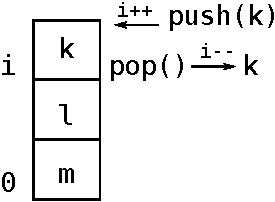
\includegraphics[scale=0.50]{fig/stack.pdf}
\end{center}
\end{wrapfigure}

\Question \label{ex:stack q2} Bonus. Write a \func{String} method which 
converts the stack to a string. This way you can print the stack using:
\lstinline{fmt.Printf("My stack %v\n", stack)}. This may aid in
debugging.
\end{Exercise}

\begin{Answer}

\Question 

\Question 

\end{Answer}


\begin{Exercise}[title={Stack as package},difficulty=2]
\label{ex:stack-package}
\Question\label{ex:stack-package q1} Create a proper package for your
stack implementation, \func{push}, \func{pop} and the \type{stack} type need to be
exported.

\Question\label{ex:stack-package q2} Which official Go package could
also be used for a (FIFO) stack?

\end{Exercise}

\begin{Answer}
\Question There are a few details that should be changed to make a proper package
for our stack. First, the exported function should begin with a capital 
letter and so should \type{Stack}. So the full package (including the
\func{String()} function becomes
\lstinputlisting[caption=Stack in a
package]{ex-functions/src/stack-as-package.go}

\Question The \package{container/vector} package would be a could candidate. It
even comes with \func{push} and \func{pop} functions \emph{predefined}.
\end{Answer}


\begin{Exercise}[title={Var args},difficulty=5]
\label{ex:varargs}
\Question\label{ex:varargs q1}
Write a function that takes a variable numbers of \type{int}s and prints
each integer on a seperate line
\end{Exercise}

\draft{BETER}
\begin{Answer}
\Question
For this we need the \lstinline{...}-syntax so signal we have a
function that takes an arbitrary number of arguments.

\lstinputlisting[label=src:varargs,caption=A function with variable number of arguments]{ex-functions/src/var-arg.go}

\end{Answer}


\begin{Exercise}[title={斐波那契},difficulty=5]
\label{ex:fibonaci}
\Question\label{ex:fibonaci q1}
斐波那契数列以:$1, 1, 2, 3, 5, 8, 13, \ldots$ 开始。
或者用数学形式表达:$ x_1 = 1; x_2 = 1; x_n = x_{n-1} +
x_{n-2}\quad\forall n > 2 $。

编写一个函数,接受 \type{int} 值,并给出这个值得到的斐波那契数列。

\end{Exercise}

\begin{Answer}
\Question
下面的程序会计算出斐波那契数列。
\lstinputlisting[label=src:fib,caption=Fibonacci function in Go]{ex-functions/src/fib.go}

\showremarks
\end{Answer}


\begin{Exercise}[title={Map function},difficulty=4]
\label{ex:map function}
A \func{map()}-function is a function that takes
a function and a list. The function is applied to 
each member in the list and a new list containing
these calculated values is returned.
Thus: 
$$ map(f(), (a_1,a_2,\ldots,a_{n-1},a_n)) =  (f(a_1), f(a_2),\ldots,f(a_{n-1}), f(a_n)) $$
\Question \label{ex:map function q1} Write a simple
\func{map()}-function in Go. It is sufficient
for this function only to work for ints.
\Question \label{ex:map function q2} Expand your code to also work on a list of strings.

\end{Exercise}

\begin{Answer}

\Question 
\begin{lstlisting}[caption=A \func{Map} function]
func Map(f func(int) int, l []int) []int {
        j := make([]int, len(l))
        for k, v := range l {
                j[k] = f(v)
        }
        return j
}

func main() {
        m := []int{1, 3, 4}
        f := func(i int) int {
                return i * i
        }
        fmt.Printf("%v", (Map(f, m)))
}
\end{lstlisting}

\Question Answer to question but now with strings
\end{Answer}




\cleardoublepage
\section{Answers}
\shipoutAnswer


\chapter{Packages}
\label{chap:packages}
\epi{"\lstinline{^}"}{\textit{Answer to whether there is a bit wise negation
operator.}\\\textsc{KEN THOMPSON}}
\noindent{}Packages are a collection of functions and data. 
You declare a package with the
\first{\key{package}}{keyword!package} keyword. The file name does not
have to match the package name.
The convention for package names is to use
lowercase characters.
Go packages may consist of multiple files,
but they share the \lstinline{package <name>} line.
Let's define a package \package{even}\index{package!even} in the file \prog{even.go}.

\lstinputlisting[label=src:even,caption=A small package]{src/even.go}
Names that start with a capital letter are \emph{exported} and may be used
outside your package, more on that later.

Now we just need to build the package. We create a directory under \var{\$GOPATH},
copy the \file{even.go} to there (see "\titleref{sec:building a program}" in chapter \ref{chap:basics}).

\begin{display}
\pr \user{mkdir $GOPATH/src/even}	\coderemark{Create top-level directory}
\pr \user{cp even.go $GOPATH/src/even} 	\coderemark{Copy the package file}
\pr \user{go build even}                \coderemark{Build it}
\end{display}

Next we can use the package in our own program \prog{myeven.go}:

\lstinputlisting[label=src:myeven,caption=Use of the even package]{src/myeven.go}
\showremarks

\begin{display}
\pr \user{go build myeven.go}
\pr \user{./myeven}
Is 5 even? false
\end{display}

In Go, a function from a package is exported (visible
outside the package, i.e. public) when the first letter of the function name is a capital, hence
the function name \func{\emph{E}ven}. If we change our \prog{myeven.go} on line
10 to using the unexported function \func{even.odd}:

\noindent\lstinline{fmt.Printf("Is %d even? %v\n", i, even.odd(i))}

We get an error when compiling, because we are trying to use a
\emph{private} function:
\begin{display}
# _/myeven
myeven.go:10: cannot refer to unexported name even.odd
\end{display}

\noindent{}To summarize:
\begin{itemize}
\item Public functions have a name starting with a \emph{capital}
letter;
\index{public}
\item Private function have a name starting with a \emph{lowercase} letter.
\index{private}
\end{itemize}
This convention also holds true for other names (new types, global
variables) you define in a package. Note that the term "capital" is not limited
to US ASCII, it extends into the entire Unicode range. So capital Greek, Coptic, etc. is OK too.

\section{Identifiers}
Names are as important in Go as in any other language. In some cases
they even have semantic effect: for instance, the visibility of a name
outside a package is determined by whether its first character is upper
case. It's therefore worth spending a little time talking about naming
conventions in Go programs.

The convention that is used was to leave well-known legacy
not-quite-words alone rather than try to figure out where
the capital letters go.  \lstinline{Atoi}, \lstinline{Getwd},
\lstinline{Chmod}.
Camelcasing works best when you have whole words
to work with: \lstinline{ReadFile, NewWriter, MakeSlice}.

\subsection{Package names}
When a package is imported (with \first{\key{import}}{keyword!import}), the package name becomes 
an accessor for the contents. After\index{package!bytes}
\begin{lstlisting}
import "bytes"
\end{lstlisting}
the importing package can talk about \func{bytes.Buffer}. It's helpful if
everyone using the package can use the same name to refer to its
contents, which implies that the package name should be good: short,
concise, and evocative. By convention, packages are given lower case,
single-word names; there should be no need for underscores or mixedCaps.
Err on the side of brevity, since everyone using your package will be
typing that name. And don't worry about collisions a priori. The package
name is only the default name for imports. With the above import 
you can use \lstinline{bytes.Buffer}. With 
\begin{lstlisting}
import bar "bytes"
\end{lstlisting}
it becomes \lstinline{bar.Buffer}.
So it does need not be unique across
all source code, and in the rare case of a collision the importing
package can choose a different name to use locally. In any case,
confusion is rare because the file name in the import determines just
which package is being used.

Another convention is that the package name is the base name of its
source directory; the package in \package{src/pkg/compress/gzip} is imported as
\var{compress/gzip} but has name \package{gzip}, not
\package{compress\_gzip} and not
\package{compressGzip}.\index{package!compress/gzip}

The importer of a package will use the name to refer to its contents, so 
exported names in the package can use that fact to avoid
stutter. For instance, the buffered reader type in the
\package{bufio}\index{package!bufio}
package is
called \func{Reader}, not \func{BufReader}, because users see it as
\func{bufio.Reader},
which is a clear, concise name. Moreover, because imported entities are
always addressed with their package name, \func{bufio.Reader} does not conflict
with \func{io.Reader}. Similarly, the function to make new instances of
\func{ring.Ring} (package \package{container/ring}) ---which is the definition of a constructor in Go---would normally
be called \func{NewRing}, but since \type{Ring} is the only type exported by the
package, and since the package is called
\package{ring}\index{package!ring}, it's called
just \func{New}.
Clients of the package see that as \func{ring.New}. Use the package structure
to help you choose good names.

Another short example is \func{once.Do} (see package \package{sync}); \func{once.Do(setup)} reads well and would
not be improved by writing \lstinline{once.DoOrWaitUntilDone(setup)}. Long names
don't automatically make things more readable. If the name represents
something intricate or subtle, it's usually better to write a helpful
doc comment than to attempt to put all the information into the name.

Finally, the convention in Go is to use \first{MixedCaps}{MixedCaps} or mixedCaps rather
than underscores to write multi-word names.

%% Advanced Go, leave it
%%\section{Initialization}
%%Every source file in a package can define an \func{init()} function. This function is
%%called after the variables in the package have gotten their value. The
%%\func{init()} function can be used to setup state before the execution
%%begins.

\section{Documenting packages}
\gomarginpar{This text is copied from \cite{effective_go}.}
Every package should have a \emph{package comment}, a block comment preceding the
\key{package} clause. For multi-file packages, the package comment only needs to be
present in one file, and any one will do. The package comment should introduce
the package and provide information relevant to the package as a whole. It will
appear first on the \prog{go doc} page and should set up the detailed documentation
that follows. An example from the official \package{regexp} package:
\begin{display}
/*
    The regexp package implements a simple library for
    regular expressions.

    The syntax of the regular expressions accepted is:

    regexp:
        concatenation { '|' concatenation }
*/
package regexp
\end{display}

Each defined (and exported) function should have a small line of text
documenting the behavior of the function. An example from the \package{fmt}
package:
\begin{display}
// Printf formats according to a format specifier and writes to standard
// output. It returns the number of bytes written and any write error
// encountered.
func Printf(format string, a ...interface{}) (n int, err error)
\end{display}

\section{Testing packages}
In Go it is customary to write (unit) tests for your package. Writing
tests involves the \package{testing} package and the program
\first{\prog{go test}}{tooling!go!test}. Both
have excellent documentation. When you include tests with your package
keep in mind that they have to build using the standard \file{Makefile}
(see section "\titleref{sec:building a package}").

%% CLEANFILES+=hello fib chain run.out
%%

The testing itself is carried out with \prog{go test}.
The \prog{go test} program runs all the test functions. Without any
defined tests for our \package{even} package, \prog{go test} yields:
\begin{display}
\pr \user{go test}
?       even    [no test files]
\end{display}
Let us fix this by defining a test in a test file. Test files reside
in the package directory and are named \file{*\_test.go}. Those test
files are just like other Go program, but \prog{go test} will only
execute the test functions.
Each test function has the same signature and its name should start
with \lstinline{Test}:
\begin{lstlisting}
func TestXxx(t *testing.T) |\coderemark{Test<Capital>restOftheName}|
\end{lstlisting}

When writing test you will need to tell \prog{go test} that a test has
failed or was successful. A successful test function just returns. When
the test fails you can signal this with the following
functions \cite{go_doc}. These are the most important ones (see \prog{go doc testing}
for more):

\begin{lstlisting}[numbers=none]
func (t *T) Fail()
\end{lstlisting}
\func{Fail} marks the test function as having failed but continues execution.

\begin{lstlisting}[numbers=none]
func (t *T) FailNow()
\end{lstlisting}
\func{FailNow} marks the test function as having failed and stops its execution.
Execution will continue at the next test. So any other test in
\emph{this} file are skipped too.

\begin{lstlisting}[numbers=none]
func (t *T) Log(args ...interface{})
\end{lstlisting}
\func{Log} formats its arguments using default formatting, analogous to
\func{Print()}, and records the text in the error log.

\begin{lstlisting}[numbers=none]
func (t *T) Fatal(args ...interface{})
\end{lstlisting}
\func{Fatal} is equivalent to \func{Log()} followed by \func{FailNow()}.

Putting all this together we can write our test. First
we pick a name: \file{even\_test.go}. Then we add the following contents:
\lstinputlisting[label=src:eventest,caption=Test file for even
package,numbers=right]{src/even_test.go}
Note that we use \lstinline{package even} on line 1, the tests fall in the same
namespace as the package we are testing. This not only convenient, but
also allows tests of unexported function and structures. We then import
the \package{testing} package and on line 5 we define the only test
function in this file. The displayed Go code should not hold any
surprises: we check if the \func{Even} function works OK. 
Now, the moment we've been waiting for, executing the test:
\begin{display}
\pr \user{go test}
ok      even    0.001s
\end{display}
\noindent{}Our test ran and reported \texttt{ok}. Success! 

To show how a failed test look we redefine our test function:
\begin{lstlisting}
// Entering the twilight zone
func TestEven(t *testing.T) {
        if Even(2) {
                t.Log("2 should be odd!")
                t.Fail()
        }   
}
\end{lstlisting}
We now get:
\begin{display}
FAIL    even    0.004s
--- FAIL: TestEven (0.00 seconds)
\qquad\qquad2 should be odd!
FAIL
\end{display}
\noindent{}And you can act accordingly (by fixing the test for instance).

\begin{lbar}
Writing new packages should go hand in hand with writing (some)
documentation and test functions. It will make your code better and it
shows that you really put in the effort.
\end{lbar}

\section{Useful packages}
The standard Go repository includes a huge number of packages and it is
even possible to install more along side your current Go installation. 
It is very enlightening to browse the \file{\$GOROOT/src/pkg} directory and
look at the packages.
We cannot comment on each package, but the following are worth a mention:
\footnote{The descriptions are copied from the packages' \prog{go doc}. Extra
remarks are type set in italic.}

\begin{description}
\item[\package{fmt}]{\index{package!fmt}
Package \package{fmt} implements formatted I/O with functions analogous
to C's \func{printf} and \func{scanf}. The format verbs are derived
from C's but are simpler. Some verbs (\%-sequences) that can be used:

\begin{description}
\item[\%v]{The value in a default format.
when printing structs, the plus flag (\%+v) adds field names;}
\item[\%\#v]{a Go-syntax representation of the value.}
\item[\%T]{a Go-syntax representation of the type of the value;}
\end{description}

}

\item[\package{io}]{\index{package!io}
This package provides basic interfaces to I/O primitives.
Its primary job is to wrap existing implementations of such primitives,
such as those in package os, into shared public interfaces that
abstract the functionality, plus some other related primitives.
}
\item[\package{bufio}]{\index{package!bufio}
This package implements buffered I/O.  It wraps an 
\lstinline{io.Reader}
or
\lstinline{io.Writer}
object, creating another object (Reader or Writer) that also implements
the interface but provides buffering and some help for textual I/O.
}
\item[\package{sort}]{\index{package!sort}
The \package{sort} package provides primitives for sorting arrays
and user-defined collections.
}
\item[\package{strconv}]{\index{package!strconv}
The \package{strconv} package implements conversions to and from
string representations of basic data types.
}
\item[\package{os}]{\index{package!os}
The \package{os} package provides a platform-independent interface to operating
system functionality.  The design is Unix-like.
}
\item[\package{sync}]{\index{package!sync}
The package \package{sync} provides basic synchronization primitives such as mutual
exclusion locks. 
}
\item[\package{flag}]{\index{package!flag}
The \package{flag} package implements command-line flag parsing. 
\emph{See "\titleref{sec:option parsing}"
on page \pageref{sec:option parsing}.}
}
\item[\package{json}]{\index{package!json}
The \package{json} package implements encoding and decoding of JSON objects as
defined in RFC 4627 \cite{RFC4627}.
}
\item[\package{template}]{\index{package!template}
Data-driven templates for generating textual output such as HTML.

Templates are executed by applying them to a data structure.  Annotations in
the template refer to elements of the data structure (typically a field of a
struct or a key in a map) to control execution and derive values to be
displayed.  The template walks the structure as it executes and the "cursor" @
represents the value at the current location in the structure.
}
\item[\package{http}]{\index{package!http}
The \package{http} package implements parsing of HTTP requests, replies,
and URLs and provides an extensible HTTP server and a basic
HTTP client.
}
\item[\package{unsafe}]{\index{package!unsafe}
The \package{unsafe} package contains operations that step around the type safety of Go programs.
\emph{Normally you don't need this package.}
}
\item[\package{reflect}]{\index{package!reflect}
The \package{reflect} package implements run-time reflection, allowing a program to
manipulate objects with arbitrary types.  The typical use is to take a
value with static type \lstinline|interface{}| and extract its dynamic type
information by calling \func{TypeOf}, which returns an object with interface
type \type{Type}.

\emph{See chapter \ref{chap:interfaces}, 
section "\titleref{sec:introspection and reflection}"}.
}
\item[\package{exec}]{\index{package!exec}
The \package{exec} package runs external commands.
}
\end{description}

\section{Exercises}
\begin{Exercise}[title={stack 包},difficulty=0]
\label{ex:stack-package}
\Question\label{ex:stack-package q1} 
参考 Q\ref{ex:stack} 练习。在这个练习中将从那个代码中建立一个独立的包。
为 stack 的实现创建一个合适的包,\func{Push}、\func{Pop} 和 \type{Stack} 类型需要被导出。

\Question\label{ex:stack-package q2} 为这个包编写一个单元测试,
至少测试 \func{Push} 后 \func{Pop} 的工作情况。

\end{Exercise}

\begin{Answer}
\Question 在创建 stack 包时,仅有一些小细节需要修改。
首先,导出的函数应当大写首字母,因此应该是 \type{Stack}。
包所在的文件被命名为 \file{stack-as-package.go},内容是:
\lstinputlisting[caption=包里的 Stack]{ex-packages/src/stack-as-package.go}

\Question 为了让单元测试正常工作,需要做一些准备。
下面用一分钟的时间来做这些。首先是单元测试本身。
创建文件 \file{pushpop\_test.go},有如下内容:
\lstinputlisting[caption=Push/Pop 测试]{ex-packages/src/pushpop_test.go}
为了让 \prog{go test} 能够工作,需要将包所在文件放到 
\var{\$GOPATH/src}:\\

\begin{display}
\pr \user{mkdir $GOPATH/src/stack}
\pr \user{cp pushpop_test.go $GOPATH/src/stack}
\pr \user{cp stack-as-package.go $GOPATH/src/stack}
\end{display}

输出:\\

\begin{display}
\pr \user{go test stack}
ok      stack   0.001s
\end{display}
\end{Answer}


\begin{Exercise}[title={Calculator},difficulty=7]
\label{ex:calc}
\Question\label{ex:calc q1} Create a reverse polish calculator. Use your
stack package.

\end{Exercise}

\begin{Answer}
\Question This is one answer:
\lstinputlisting[caption=A (rpn) calculator]{ex-packages/src/calc.go}

\end{Answer}


\cleardoublepage
\section{Answers}
\shipoutAnswer


\chapter{Beyond the basics}
\label{chap:beyond}
\epi{\lstinline{fmt.Printf("\%p", i)}}{Printing the address of a pointer in Go.}
\noindent{}
\subsection{Nil value}
A reference to nothing is represented in Go as \lstinline{nil}. This is
different than a zero value. \todo{nil only for references?}

\begin{lstlisting}
var *a int
a = nil
fmt.Printf("%v\n", a);
\end{lstlisting}
Prints \lstinline{nil}.

\section{Conversions}
\label{sec:conversions}
Sometimes you want to convert a type to another type. In C this is known
as casting a value to another type. This is also possible in Go, but
there are some rules.\todo{there are more rules, but we're trying to
keep it simple...}
You can convert:
\begin{itemize}
\item{
From a \lstinline{string} to a slice of \lstinline{byte}s.
\begin{lstlisting}
mystring = "hello this is string"
byteslice =  []byte(mystring)
\end{lstlisting}
}
\item{
From a slice of \lstinline{byte}s to a \lstinline{string}.
\begin{lstlisting}
The other way around
\end{lstlisting}
}
\end{itemize}
\todo{Maybe put this to the end of this chapter}
%%x is an integer or has type []byte or []int and T is a string type.
%%and back
%% integer/float truncation














You may have wished otherwise, but Go has pointers.
There is however now pointer arithmetic and they are still useful.
Remember Go when you call a function in Go the variables you pass are
pass-by-value. So, for efficiency and the possibility to modify a
passed value \emph{in} the function we have pointers.

%% Do we need a whole chapter on Pointers in Go
Just like in C you declare a pointer by prefixing the type with an `*`,
so:

are declared after variable names, and all type modifiers precede the
\todo{}%
types. So *X is a pointer to an X; [3]X is an array of three X's. The
types are therefore really easy to read just read out the names of the
type modifiers: [] declares something called an array slice; "*"
declares a pointer; [size] declares an array. So []*[3]*int is an array
slice of pointers to arrays of three pointers to ints

\noindent\lstinline{var pint *int   // declare pint to be pointer to int}

Note that it's perfectly OK to return the address of a local variable; the
storage associated with the variable survives after the function returns. In
fact, taking the address of a composite literal allocates a fresh instance each
time it is evaluated, so we can combine these last two lines. \cite{effective_go}

\section{Allocation}
Go has garbage collection, meaning that you don't have to worry about
memory allocation and deallocation. Of course almost every language
since 1980 has this, but it is nice to see garbage collection in a
C-like language. The following sections show how to handle allocation
in Go. There is somewhat an artifical distinction between
\first{\func{new()}} and \first{\func{make()}}. Details follow.

\section{Allocation with \func{new()}}
Go has two allocation primitives, \func{new()} and \func{make()}. They do different
things and apply to different types, which can be confusing, but the
rules are simple. Let's talk about \func{new()} first. It's a built-in function
essentially the same as its namesakes in other languages: \func{new(T)}
allocates zeroed storage for a new item of type \type{T} and returns its
address, a value of type \type{*T}. In Go terminology, it returns a pointer to
a newly allocated zero value of type \type{T}.

Since the memory returned by \func{new()} is zeroed, it's helpful to arrange
that the zeroed object can be used without further initialization. This
means a user of the data structure can create one with \func{new()} and get
right to work. For example, the documentation for \type{bytes.Buffer} states
that "the zero value for Buffer is an empty buffer ready to use."
Similarly, \func{sync.Mutex} does not have an explicit constructor or Init
method. Instead, the zero value for a \func{sync.Mutex} is defined to be an
unlocked mutex.

The zero-value-is-useful property works transitively. Consider this type
declaration.

\begin{lstlisting}
type SyncedBuffer struct {
    lock    sync.Mutex
    buffer  bytes.Buffer
}
\end{lstlisting}
Values of type \type{SyncedBuffer} are also ready to use immediately upon
allocation or just declaration. In this snippet, both \var{p} and
\var{v} will work
correctly without further arrangement.
\begin{lstlisting}
p := new(SyncedBuffer)  // type *SyncedBuffer
var v SyncedBuffer      // type  SyncedBuffer
\end{lstlisting}

\section{Constructors and composite literals}
Sometimes the zero value isn't good enough and an initializing
constructor is necessary, as in this example derived from package
\package{os}.
\begin{lstlisting}
func NewFile(fd int, name string) *File {
    if fd < 0 {
        return nil
    }
    f := new(File)
    f.fd = fd
    f.name = name
    f.dirinfo = nil
    f.nepipe = 0
    return f
}
\end{lstlisting}
There's a lot of boiler plate in there. We can simplify it using a
composite literal, which is an expression that creates a new instance
each time it is evaluated.

\begin{lstlisting}
func NewFile(fd int, name string) *File {
    if fd < 0 {
        return nil
    }
    f := File{fd, name, nil, 0}
    return &f
}
\end{lstlisting}
Note that it's perfectly OK to return the address of a local variable;
the storage associated with the variable survives after the function
returns. In fact, taking the address of a composite literal allocates a
fresh instance each time it is evaluated, so we can combine these last
two lines.

\begin{lstlisting}
return &File{fd, name, nil, 0}
\end{lstlisting}
The fields of a composite literal are laid out in order and must all be
present. However, by labeling the elements explicitly as field:value
pbairs, the initializers can appear in any order, with the missing ones
left as their respective zero values. Thus we could say

\begin{lstlisting}
return &File{fd: fd, name: name}
\end{lstlisting}
As a limiting case, if a composite literal contains no fields at all, it
creates a zero value for the type. The expressions
\lstinline{new(File)} and 
\lstinline|&File{]| are equivalent.

Composite literals can also be created for arrays, slices, and maps,
with the field labels being indices or map keys as appropriate. In these
examples, the initializations work regardless of the values of Enone,
Eio, and Einval, as long as they are distinct.
\begin{lstlisting}
a := [...]string   {Enone: "no error", Eio: "Eio", Einval: "invalid argument"}
s := []string      {Enone: "no error", Eio: "Eio", Einval: "invalid argument"}
m := map[int]string{Enone: "no error", Eio: "Eio", Einval: "invalid argument"}
\end{lstlisting}

\section{Allocation with \func{make()}}
Back to allocation. The built-in function \func{make(T, args)} serves a purpose
different from \func{new(T)}. It creates slices, maps, and channels only, and
it returns an initialized (not zero) value of type T, not *T. The reason
for the distinction is that these three types are, under the covers,
references to data structures that must be initialized before use. A
slice, for example, is a three-item descriptor containing a pointer to
the data (inside an array), the length, and the capacity; until those
items are initialized, the slice is nil. For slices, maps, and channels,
make initializes the internal data structure and prepares the value for
use. For instance,
\lstinline{make([]int, 10, 100)}
allocates an array of 100 ints and then creates a slice structure with
length 10 and a capacity of 100 pointing at the first 10 elements of the
array. (When making a slice, the capacity can be omitted; see the
section on slices for more information.) In contrast, new([]int) returns
a pointer to a newly allocated, zeroed slice structure, that is, a
pointer to a nil slice value.

These examples illustrate the difference between new() and make().
\begin{lstlisting}
var p *[]int = new([]int)       // allocates slice structure; *p == nil; rarely useful
var v  []int = make([]int, 100) // v now refers to a new array of 100 ints

// Unnecessarily complex:
var p *[]int = new([]int)
*p = make([]int, 100, 100)

// Idiomatic:
v := make([]int, 100)
\end{lstlisting}
Remember that make() applies only to maps, slices and channels and does
not return a pointer. To obtain an explicit pointer allocate with new().


\section{Defining your own}
\label{sec:defining your own}
Ofcourse Go allows you to define new types, it does this in (almost) the
same way as in C, with the \key{struct} keyword.

An empty struct is created with \lstinline|var empty struct {}|{}.
A more real-life example would be when we want record seomebody's name
and age in a single ... TODO. We could do

\lstinputlisting[label=src:struct,caption=Structures]{src/struct.go}

Apropos, the output of \lstinline{fmt.Printf("\%v\n", a)} is 
\begin{display}
{Pete, 42}
\end{display}
How nice is that, Go knows how to print your structure! If you
only want to print a one, or a few, field of the structure you'll
need to use \verb|<field name>|. To only print the name:
\begin{lstlisting}
fmt.Printf("%v", a.name)
\end{lstlisting}

Defining a new type:

\begin{lstlisting}
type T struct {
    name string // name of the object
    value int // its value
}
\end{lstlisting}

Or alias a build in one.
Methods on types, and methods on build in type - can not do that,
just create a new type.

\section{Exercises}
\begin{Exercise}[title={指针},difficulty=6]
\label{ex:pointers}

\Question
假设定义了下面的结构:
\begin{lstlisting}
type Person struct {
    name string
    age	 int
}
\end{lstlisting}

下面两行之间的区别是什么?
\begin{lstlisting}
var p1 Person
p2 := new(Person)
\end{lstlisting}

\Question
下面两个内存分配的区别是什么?
\begin{lstlisting}[numbers=none]
func Set(t *T) {
    x = t
}
\end{lstlisting}
和
\begin{lstlisting}[numbers=none]
func Set(t T) {
    x= &t
}
\end{lstlisting}
\end{Exercise}

\begin{Answer}
\Question
第一行:\lstinline{var p1 Person} 分配了
\texttt{Person}-\emph{值} 给 \var{p1}。\var{p1} 的类型是
\type{Person}。

第二行:\lstinline{p2 := new(Person)} 分配了内存并且将\emph{指针}赋值给
\var{p2}。\var{p2} 的类型是 \type{*Person}。

\Question
在第二个函数中,\var{x} 指向一个新的(堆上分配的)变量
\var{t},其包含了实际参数值的副本。

在第一个函数中,\var{x} 指向了 \var{t} 指向的内容,
也就是实际上的参数指向的内容。

因此在第二个函数,我们有了``额外''的变量存储了相关值的副本。
\end{Answer}


\begin{Exercise}[title={Linked List},difficulty=1]
\label{ex:linkedlist}
\Question
\label{ex:linkedlist q1}
Make use of the package \package{container/list} to create
a (double) linked list. Push the values 1, 2 and 4 to the list and then
print it.

\Question
Create your own linked list implementation. And perform the same actions
as in question \ref{ex:linkedlist q1}
\end{Exercise}

\begin{Answer}
\Question

\Question
\end{Answer}


\cleardoublepage
\section{Answers}
\shipoutAnswer


\chapter{Concurrency}
\label{chap:channels}
\epi{%
\begin{itemize}
\item{“并行是关于性能的;}
\item{并发是关于程序设计的。”}
\end{itemize}%
}{\textit{Google IO 2010}\\\textsc{ROBE PIKE}}
\noindent{}在这章中将展示 Go 使用 channel 和 goroutine 开发并行程序的能力。
goroutine 是 Go 并发能力的核心要素。但是,goroutine 到底 \emph{是}什么?来自
\cite{effective_go}:
\begin{quote}
叫做 goroutine 是因为已有的短语——线程、协程、进程等等——传递了不准确的含义。
goroutine 有简单的模型:\emph{它是与其他 goroutine 并行执行的,有着相同地址空间的函数。}。
它是轻量的,仅比分配栈空间多一点点消耗。而初始时栈是很小的,所以它们也是廉价的,
并且随着需要在堆空间上分配(和释放)。
\end{quote}
\first{goroutine}{goroutine} 是一个普通的函数,只是需要使用保留字
\first{\key{go}}{keyword!go} 作为开头。
\begin{lstlisting}
ready("Tea", 2)	    |\coderemark{普通函数调用}|
go ready("Tea", 2)  |\coderemark{\func{ready()} 作为 goroutine 运行}|
\end{lstlisting}
下面程序的思路来自 \cite{go_course_day3}。
让一个函数作为两个 goroutine 执行,goroutine 等待一段时间,然后打印一些内容到屏幕。
在第 14 和 15 行,启动了 goroutine。
\func{main} 函数等待足够的长的时间,这样每个 goroutine 会打印各自的文本到屏幕。
现在是在第 17 行等待 5 秒钟(\func{time.Sleep()} 按 ns 计算),、
但实际上没有任何办法知道,当所有 goroutine 都已经退出应当等待多久。 
\lstinputlisting[numbers=right,label=src:sleeping,firstnumber=8,caption=Go routine 实践,linerange={8,18}]{src/sleep.go}
表 \ref{src:sleeping} 输出:
\begin{display}
I'm waiting         \coderemark{立刻}
Coffee is ready!    \coderemark{1 秒后}
Tea is ready!       \coderemark{2 秒后}
\end{display}
如果不等待 goroutine 的执行(例如,移除第 17 行),程序立刻终止,而任何正在执行的 
goroutine 都\emph{会停止}。
为了修复这个,需要一些能够同 goroutine 通讯的机制。这一机制通过 \first{channels}{channels} 
的形式使用。\first{channel}{channel} 可以与 Unix sehll 中的双向管道做类比:
可以通过它发送或者接收值。这些值只能是特定的类型:channel 类型。
定义一个 channel 时,也需要定义发送到 channel 的值的类型。注意,必须使用
\key{make} 创建 channel:
\begin{lstlisting}
ci := make(chan int)
cs := make(chan string)
cf := make(chan interface{})
\end{lstlisting}
创建 channel \var{ci} 用于发送和接收整数,创建 channel \var{cs} 用于字符串,
以及 channel \var{cf} 使用了空接口来满足各种类型。
向 channel 发送或接收数据,是通过类似的操作符完成的:
\lstinline{<-}. \index{operator!channel}
具体作用则依赖于操作符的位置:
\begin{lstlisting}
ci <- 1	    |\coderemark{\emph{发送}整数 1 到 channel \var{ci}}|
<-ci	    |\coderemark{从 channel \var{ci} \emph{接收}整数}|
i := <-ci   |\coderemark{从 channel \var{ci} \emph{接收}整数,并保存到 \var{i} 中}|
\end{lstlisting}
将这些放到实例中去。
\begin{lstlisting}[numbers=none,caption=Go routines 和 channel,label=src:sleeping with channels]
var c chan int |\longremark{定义 \var{c} 作为 int 型的 channel。就是说:这个 channel 传输整数。%
注意这个变量是全局的,这样 goroutine 可以访问它;}|

func ready(w string, sec int) {
	time.Sleep(int64(sec) * 1e9)
	fmt.Println(w, "is ready!")
	c <- 1	|\longremark{发送整数 1 到 channel \var{c};}|
}

func main() {
	c = make(chan int) |\longremark{初始化 \var{c};}|
	go ready("Tea", 2) |\longremark{用保留字 \key{go} 开始一个 goroutine;}|
	go ready("Coffee", 1)
	fmt.Println("I'm waiting, but not too long")
	<-c |\longremark{等待,直到从 channel 上接收一个值。注意,收到的值被丢弃了;}|
	<-c |\longremark{两个 goroutines,接收两个值。}|
}
\end{lstlisting}

\showremarks
这里仍然有一些丑陋的东西;不得不从 channel 中读取两次(第 14 和 15 行)。
在这个例子中没问题,但是如果不知道有启动了多少个 goroutine 怎么办呢?
这里有另一个 Go 内建的保留字:\first{\key{select}}{keyword!select}。
通过 \key{select}(和其他东西)可以监听 channel 上输入的数据。

在这个程序中使用 \key{select},并不会让它变得更短,因为运行的 go\-routine 太少了。
移除第 14 和 15 行,并用下面的内容替换它们:
\begin{lstlisting}[caption=使用 select,numbers=right,firstnumber=14]
L: for {
	select {
	case <-c:
		i++ 
		if i > 1 { 
			break L
		}   
	}   
}   
\end{lstlisting}

\subsection{使其并行运行}
虽然 goroutine 是并发执行的,但是它们并不是并行运行的。如果不告诉 Go 额外的东西,
同一时刻只会有一个 goroutine 执行。利用 \func{runtime.GOMAXPROCS(n)} 可以设置 goroutine 并行执行的数量。
来自文档:
\begin{quote}
GOMAXPROCS 设置了同时运行的 CPU 的最大数量,并返回之前的设置。如果 n < 1,不会改变当前设置。
\emph{当调度得到改进后,这将被移除。}
\end{quote}
如果不希望修改任何源代码,同样可以通过设置环境变量
 \verb|GOMAXPROCS| 为目标值。
%% test
%%\marginpar{%
%%$$\left\{
%%\begin{array}{l}
%%\parbox{2cm}{
%%hallo Yppp hallo Yppp hallo Yppp
%%hallo Yppp hallo Yppp hallo Yppp
%%hallo Yppp
%%}
%%\end{array}
%%\right.$$
%%}

%%\section{So many channels and still \ldots}
\section{更多关于 channel}
\label{sec:more on channels}
当在 Go 中用 \lstinline{ch := make(chan bool)} 创建 chennel 时,bool 型的
\first{无缓冲 channel}{channel!unbuffered} 会被创建。
这对于程序来说意味着什么呢?首先,如果读取(\lstinline{value := <-ch})它将会被阻塞,直到有数据接收。
其次,任何发送(\lstinline{ch<-5}) 将会被阻塞,直到数据被读出。
无缓冲 channel 是在多个 goroutine 之间同步很棒的工具。
\index{channel!blocking read}
\index{channel!blocking write}

不过 Go 也允许指定 channel 的缓冲大小,很简单,就是 channel 可以存储多少元素。
\lstinline{ch := make(chan bool, 4)},创建了可以存储 4 个元素的 bool 型 channel。
在这个 channel 中,前 4 个元素可以无阻塞的写入。当写入第 5$^{个}$ 元素时,代码
\emph{将会}阻塞,直到其他 goroutine 从 channel 中读取一些元素,腾出空间。
\index{channel!non-blocking read}
\index{channel!non-blocking write}

虽然从 channel 读取是阻塞的,但是仍然可以用下面的方式实现非阻塞的读取:
\todo{需要对这个做一些测试。}
\begin{lstlisting}
x, ok = <-ch
\end{lstlisting}
当读取到了内容时 \lstinline{ok} 为 \lstinline{true},否则为 \lstinline{false}。
同时,\lstinline{x} 从 channel 获取到值。
一句话说,在 Go 中下面的为 true:
$$
\textrm{\lstinline{ch := make(chan type, value)}}
\left\{
\begin{array}{ll}
value == 0 & \rightarrow \textrm{无缓冲(阻塞)} \\
value >  0 & \rightarrow \textrm{缓冲(非阻塞,直到 \emph{value} 个元素)}
\end{array}
\right.
$$

\subsection{关闭 channel}
%% section needs to be written

\subsection{在 goroutines 中包装函数}
参阅 godns/resolver.go 如何在 goroutine 中用错误处理等包装 Query() 函数。

\section{练习}
\begin{Exercise}[title={Channel},difficulty=4]
\label{ex:channels}
\Question\label{ex:channels q1} 修改在练习 Q\ref{ex:for-loop} 中创建的程序,
换句话说,主体中调用的函数现在是一个 goroutine 并且使用 channel 通讯。
不用担心 goroutine 是如何停止的。

\Question\label{ex:channels q2} 在完成了问题 \ref{ex:channels q1} 后,仍有一些待解决的问题。
其中一个麻烦是 goroutine 在 \func{main.main()} 结束的时候,没有进行清理。
更糟的是,由于 \func{main.main()} 和 \func{main.shower()} 的竞争关系,不是所有数字都被打印了。
本应该打印到 9,但是有时只打印到 8。添加第二个退出 channel,可以解决这两个问题。试试吧。
\footnote{需要用到 \func{select} 语句。}

\end{Exercise}

\begin{Answer}
\Question 程序可能的形式是: 
\lstinputlisting[label=go-chan,caption=Go 的 channel,numbers=right]{ex-channels/src/for-chan.go}
以通常的方式开始,在第 6 行创建了一个新的 int 类型的 channel。下一行调用了
\func{shower} 函数,用 \prog{ch} 变量作为参数,这样就可以与其通讯。然后进入 for 循环(第 8-10 行),
在循环中发送(通过 \lstinline{<-})数字到函数(现在是 goroutine)\func{shower}。
在函数 \func{shower} 中等待(阻塞方式),直到接收到了数字(第 15 行)。
每个收到的数字都被打印(第 16 行)出来,然后继续第 14 行开始的死循环。

\Question 答案是
\lstinputlisting[label=go-quit-chan,caption=添加额外的退出 channel,numbers=right]{ex-channels/src/for-quit-chan.go}
在第 20 行从退出 channel 读取并丢弃该值。可以使用 \lstinline{q := <-quit},
但是可能只需要用这个变量一次——在 Go 中是非法的。另一种办法,你可能已经想到了:
\lstinline{_ = <-quit}。在 Go 中这是合法的,但是第 20 行的形式在 Go 中更好。
\end{Answer}


\begin{Exercise}[title={Fibonaci II},difficulty=7]
\label{ex:fibonaci II}
\Question\label{ex:fibonaci II q1}
This is the same exercise as the one given page \pageref{ex:fibonaci} 
in exercise \ref{ex:fibonaci}. For completeness the complete question:

\begin{quote}
The Fibonaci sequence starts as follows: $1, 1, 2, 3, 5, 8, 13, \ldots$
Or in mathematical terms: $ x_1 = 1; x_2 = 1; x_n = x_{n-1} +
x_{n-2}\quad\forall n > 2 $.

Write a function that takes an \type{int} value and gives to
Fibonaci sequence up to that value.
\end{quote}

\begin{lbar}
\emph{But} now the twist: You must use channels.
\end{lbar}


\end{Exercise}

\begin{Answer}
\Question
The following program calculates the Fibonaci numbers using channels.
\lstinputlisting[label=src:fib II,caption=A Fibonaci function in Go]{ex-channels/src/fib.go}
\end{Answer}




\cleardoublepage
\section{答案}
\shipoutAnswer


\appendix
\chapter{Expression versus statement}
\label{chap:expression}
\section{Expression versus statement}
\label{sec:expression versus statement}
In this book we talk about expressions and statements, but%
\gomarginpar{This section comes from \cite{so_expression_vs_statement}.}
what \emph{is} the difference between the two?
In short:
\begin{description}
\item[Expression] Something which evaluates to a value, like:
\lstinline{1+2/x} ;
\item[Statement] A line of code which does something, like
\lstinline{goto Error} .
\end{description}

The distinction was crystal-clear in the earliest general-purpose
programming languages, like FORTRAN. In FORTRAN, a statement was one
unit of execution: "a thing that you did". 
An expression on its own couldn't do anything. You had to assign it to a
variable.
\begin{display}
1 + 2 / X
\end{display}
is an error in FORTRAN, because it doesn't do anything. You had to do
something with that expression: 
\begin{display}{X = 1 + 2 / X}\end{display}

The earliest popular language to blur the lines was C. The designers of
C realized that no harm was done if you were allowed to evaluate an
expression and throw away the result. In C, every expression could be a
statement: 
\begin{display}1 + 2 / x\end{display}
is a totally legit statement even though absolutely nothing will happen.
Why? Because in C, expressions could have side-effects --- they could
change something: \begin{display}{1 + 2 / callfunc(12)}\end{display}

Because \func{callfunc()} might just do something useful.
Once you allow any expression to be a statement, you might as well allow
the assignment operator (=) inside expressions. That's why C lets you do
things like: \lstinline{callfunc(x = 2)}.
This evaluates the expression \lstinline{x = 2} (assigning the value of 2 to x) and
then passes that (the 2) to the function \func{callfunc()}.

This blurring of expressions and statements occurs in all the
C-derivatives (C, C++, C\#, Java and of course Go), which still have some
statements (like \key{while}) but which allow almost any expression to be used
as a statement. Functional languages like Lisp don't have statements.
All they have is expressions. 


\chapter{Colophon}
\noindent{}This work was created with \LaTeX. The main text is set in
the Google Droid fonts. All typewriter text is typeset in DejaVu Mono.

\section{Contributors}
The following people have helped to make this book what it is today.
\begin{itemize}
\item{Miek Gieben \qquad\url{<miek@miek.nl>}};
\item{JC van Winkel}.
%%\item{Filip Zaludek}.
%%\item{Jeroen Bulten}
\end{itemize}

Help with proof reading, checking exercises and text improvements (no
particular order):
\emph{Filip Zaludek},
\emph{Jonathan Kans},
\emph{Jaap Akkerhuis},
\emph{Mayuresh Kathe},
\emph{Makoto Inoue},
\emph{Ben Bullock},
\emph{Bob Cunningham},
\emph{Dan Kortschak},
\emph{Sonia Keys},
\emph{Babu Sreekanth},
\emph{Haiping Fan},
\emph{Cecil New},
and \emph{Russel Winder}.

\subsection{Miek Gieben}

\includegraphics[width=3cm]{fig/avatar-miekg-300x300}

Miek Gieben 从荷兰内梅亨大学取得计算机科学硕士学位。
他参与并开发了 DNSSEC 协议——下一代DNS——DNSSEC protocol 以及如核心认证\cite{RFC4641}。
在玩过了 Erlang 后,Go 是他当前迷恋的主要语言。
他将所有业余时间用来对 Go 的探索和编码。他是 Go DNS 库的维护者:\url{https://github.com/miekg/godns}。
他的个人博客是 \url{http://www.miek.nl} 以及 Twitter 帐号 \texttt{@miekg}。博文和推多数情况下都是关于 Go 的。



\chapter{Index}
\printindex
\bibliographystyle{plain}
\bibliography{go}
\newpage
\thispagestyle{empty}
\begin{center}
\emph{This page is intentionally left blank.}
\end{center}
\end{document}
